\chapter{Implementasi dan Pengujian}
\label{chapter:implementasi-dan-pengujian}
Bab ini akan memaparkan implementasi yang dilakukan beserta hasil evaluasi uji coba yang dilakukan. Tujuannya sebagai memberikan hasil utama dari penelitian tugas akhir ini.

\section{Lingkungan}
\label{sec:environment}

Pengembangan sistem \textit{distributed key-value store database} dilakukan pada lingkungan komputer lokal dalam \textit{virtual machine}. Berikut merupakan penjelasan implementasi dari masing-masing bagian secara terperinci yang menjadi dua bagian, yaitu perangkat lunak dan perangkat keras. Pengembangan dilakukan pada \textit{virtual machine} karena sistem memiliki pustaka yang tidak tersedia pada sistem operasi yang digunakan pada komputer lokal. Selain itu, \textit{virtual machine} juga memberikan kemudahan untuk mengatur konfigurasi sistem yang dibutuhkan untuk pengembangan sistem ini tanpa mempengaruhi sistem operasi utama yang digunakan pada komputer lokal.

Seperti yang dijelaskan pada bagian \ref{subsubsection:pilihan-bahasa-pemrograman}, implementasi \textit{distributed key-value store database} dibuat dengan menggunakan bahasa pemrograman Rust dan menggunakan pustaka bahasa tersebut. Masing-masing node dalam sistem berjalan dalam sebuah proses yang terpisah. Walaupun begitu, komunikasi antar node dilakukan dengan \textit{socket} menggunakan protokol \textit{TCP} sehingga setiap node dapat berjalan pada komputer yang berbeda jika diperlukan.

\begin{enumerate}
  \item \textbf{Perangkat Keras}
    \begin{enumerate}
      \item Prosesor: AMD Ryzen 7 5800H
      \item Memori: 64 GB RAM
      \item Penyimpanan: M.2 NVMe SSD 2 TB
    \end{enumerate}
  \item \textbf{Perangkat Lunak}
    \begin{enumerate}
      \item Sistem Operasi \textit{Host}: Windows 11 Home x64 Build 26100.4349
      \item Virtual Machine:
      \begin{enumerate}
        \item Sistem Operasi \textit{Guest}: Debian 12 Bookworm (Version 12.10)
        \item Virtualization: VMWare Workstation 17 Pro
        \item Alokasi Virtual CPU: 12 vCPU
        \item Alokasi Memori Virtual: 52 GB RAM
        \item Alokasi Penyimpanan Virtual: 250 GB
      \end{enumerate}
      \item Bahasa Pemrograman:
      \begin{enumerate}
        \item Rust (Versi: 1.84.1 linux)
        \item Bash (Versi: 5.2.15(1)-release)
        \item Javascript (Versi Node.js: v22.11.0)
      \end{enumerate}
      \item Dependensi Rust:
      \begin{enumerate}
        \item bincode (versi: 1.3.3)
        \item tokio (versi: 1, fitur: full)
        \item serde (versi: 1.0, fitur: derive)
        \item actix web (versi: 4.10.2)
        \item tracing (versi: 0.1)
        \item tracing-subscriber (versi: 0.3)
        \item tracing-appender (versi: 0.2)
        \item clap (versi: 4, fitur: derive)
        \item moka (versi: 0.12, fitur: future)
        \item rand (versi: 0.9.1)
        \item rocksdb (versi: 0.21.0)
      \end{enumerate}
      \item Dependensi Javascript:
      \begin{enumerate}
        \item k6 (Versi: 1.0.0)
      \end{enumerate}
      \item Dependensi lainnya:
      \begin{enumerate}
        \item GNU screen (Versi: 4.09.0)
        \item jq (Versi: 1.6)
        \item iptables (Versi: 1.8.7)
        \item tc (dari paket iproute2) (Versi: 5.15.0)
        \item sysstat (mpstat) (Versi: 12.5.2)
      \end{enumerate}
    \end{enumerate}
\end{enumerate}

\section{Implementasi}

Bagian ini menjelaskan tentang implementasi PERISAI secara terperinci. Seperti yang telah dijelaskan pada bagian \ref{sec:rancangan-dashboard} dan \ref{sec:rancangan-service} terdapat dua komponen utama yaitu \textit{dashboard} dan \textit{service}. Penjelasan bagian ini dimulai dari batasan implementasi, dilanjutkan dengan kakas yang digunakan dalam proses pembuatan sistem dan diakhiri dengan penjelasan mengenai implementasi dari \textit{dashboard} dan \textit{service}.

Karena PERISAI berada pada dunia IoT dan Kubernetes, perlu dilakukan pencocokan terminologi untuk memudahkan pengembangan sistem. Istilah \textit{node} pada kuberntes akan berpadanan dengan perangkat di IoT pada bagian "thing". \textit{eployment} pada kubernetes berpadanan dengan aplikasi yang dijalankan pada "thing". Kapabilitas serta tipe dari perangkat pada IoT akan dibuat menjadi label pada kubernetes.

\subsection{Batasan Implementasi}
Berikut adalah batasan yang ditetapkan dalam melakukan implementasi \textit{sistem remote deployment}.

\begin{enumerate}
  \item Semua batasan masalah dan konfigurasi yang telah dibahas pada bagian \ref{sec:batasan-masalah}.
  \item \textit{Platform agnostic} berarti PERISAI dapat dijalankan pada berbagai perangkat yang dapat menjalankan kubernetes.
  \item Kubernetes cluster berjalan di lokal dengan menggunakan kakas \textit{kind} dan hanya dibatasi menjadi 4 node dengan spesifikasi \textit{1 master} dan \textit{3 worker}
  \item \textit{Device} sudah terkoneksi sebelumnya sehingga tidak perlu register perangkat sebagai \textit{node} dan menghubungkannya ke dalam \textit{cluster}.
  \item \textit{Dashboard} hanya memilki fungsionalitas untuk \textit{user}
  \item Kubernetes memiliki batasan cluster sebagai berikut:
        \begin{enumerate}
          \item Maksimal 5000 nodes
          \item Maksimal 110 pods untuk setiap node
          \item Maksimal 150,000 total pods
          \item Maksimal 300,000 total containers
        \end{enumerate}
\end{enumerate}

\subsection{Kakas yang Digunakan}
Dalam melakukan implementasi ini diperlukan beberapa kakas, diantaranya adalah sebagai berikut.
\begin{enumerate}
  \item \textit{Docker}, \textit{Docker Desktop} dan \textit{Kind} untuk dipakai sebagai \textit{containerization} dan \textit{cluster} kubernetes lokal.
  \item Implementasi \textit{service} bahasa pemrograman golang dan menggunakan beberapa kakas berikut
        \begin{enumerate}
          \item \textit{Kubernetes Go Client} untuk mengontrol \textit{cluster} kubernetes melalui kode Golang.
          \item \textit{Echo} sebagai \textit{server framework}
          \item \textit{Logrus} sebagai logger dari setiap aksi pada sistem
          \item \textit{Cobra dan Viper} sebagai \textit{CLI command} pada golang untuk memudahkan pemilihan \textit{entrypoint} dan \textit{environment variables}
          \item \textit{PQ, Sqlx, Go-migrate} sebagai kakas yang menghubungkan sistem dengan \textit{database}. Sqlx merupakan ekstensi dari library \textit{database/sql} milik golang. Go migrate digunakan untuk melakukan migrasi dari schema sql yang telah dibuat dan melakukan keep track dari versi schema yang sedang digunakan
          \item \textit{Validator} digunakan untuk memvalidasi \textit{request} yang masuk
        \end{enumerate}

  \item Implementasi \textit{dashboard} menggunakan \textit{vue} dan \textit{typescript} dan \textit{nuxt} sebagai framework.
        \begin{enumerate}
          \item \textit{NuxtUI} Sebagai kakas untuk memudahkan pembuatan \textit{UI}.
          \item \textit{Pinia} Sebagai kakas untuk manajemen data \textit{UI}.
          \item \textit{Zod} Sebagai object schema validator sebelum mengirimkan request.
        \end{enumerate}
\end{enumerate}

\subsection{Persiapan \textit{kubernetes cluster}}
\label{subsec:persiapan-kubernetes-cluster}

Tahapan ini merupakan tahapan persiaspan sebelum proses \textit{development}. Pada tahapan ini dibuat kubernetes \textit{cluster} pada komputer lokal dengan kakas \textit{kind}. \textit{Cluster} yang dibuat memiliki 4 nodes dengan spesifikasi 1 \textit{master node} dan 3 \textit{worker node}. Digunakan \textit{command} kind create cluster --config cluster.yaml dengan file konfigurasi yang dapat dilihat pada gambar \ref{fig:konfigurasi-pembuatan-cluster}. Setelah berhasil di \textit{apply}, muncul 4 buah kontainer yang dapat berfungsi sebagai \textit{kubernetes cluster} seperti pada gamabar \ref{fig:hasil-cluster-kind}.

\begin{figure}[ht]
  \centering
  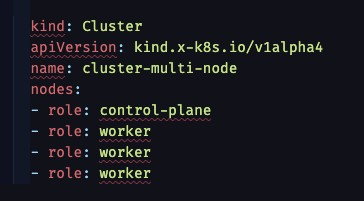
\includegraphics[width=1\textwidth]{resources/appendix/pembuatan-cluster.jpg}
  \caption{Konfigurasi Pembuatan \textit{Kubernetes Cluster} dengan \textit{Kind}}
  \label{fig:konfigurasi-pembuatan-cluster}
\end{figure}

\begin{figure}[ht]
  \centering
  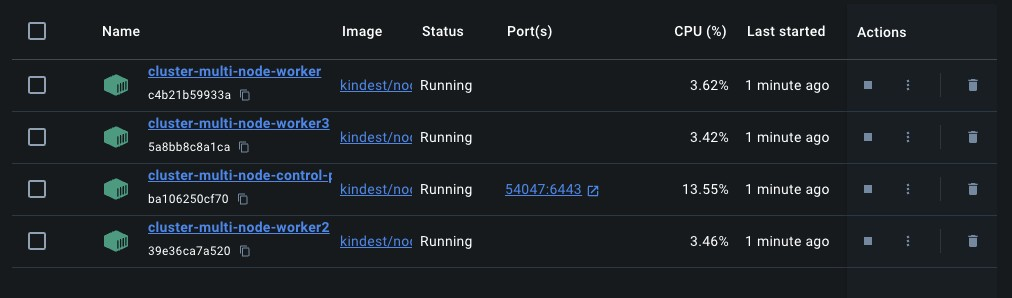
\includegraphics[width=1\textwidth]{resources/chapter-4/cluster-kind.jpg}
  \caption{Hasil \textit{Kubernetes Cluster} Dengan Kakas \textit{Kind}}
  \label{fig:hasil-cluster-kind}
\end{figure}

\pagebreak

\subsection{Implementasi \textit{Dashboard}}
Komponen \textit{dashboard} dibuat dengan menggunakan bahasa pemrogramman \textit{typescript} dan \textit{vue}. Framework yang digunakan dalam membuat \textit{Dashboard} adalah \textit{Nuxt}. \textit{Nuxt} menjadi pilihan karena memiliki \textit{developer experience} yang bagus serta fitur yang cukup lengkap. \textit{Nuxt} juga memiliki \textit{UI library} yaitu \textit{NuxtUI} yang memudahkan pembuatan \textit{UI}. Pada komponen ini, terdapat 10 halaman yang dapat dikunjungi oleh \textit{user}. Detail dari penjelasan setiap halaman dapat ditemukan pada subbab dibawah ini.

\subsubsection{Halaman \textit{Login}}
Halaman ini berada pada \textit{route} /login. Halaman ini yang berfungsi sebagai \textit{entrypoint} dari komponen \textit{dashboard}. Pada halaman ini terdapat dua input yang di \textit{wrap} oleh sebuah \textit{form}. Input berupa \textit{email} dan \textit{password} \textit{user}. Setelah \textit{user} memasukan \textit{email} dan \textit{password} yang sesuai, maka dilakukan \textit{redirect} ke laman utama untuk menunjukan bahwa \textit{user} berhasil terautentikasi dan menggunakan fungsionalitas \textit{dashboard}. Tampilan halaman ini dapat dilihat pada lampiran \ref{fig:halaman-login}.

\subsubsection{Halaman utama}
Halaman ini merupakan halaman utama dari komponen \textit{dashboard}. Pada halaman ini \textit{user} dapat melihat status dari masing masing objek mulai dari \textit{deployment}, \textit{device}, \textit{group}, serta \textit{quick actions} untuk menuju halaman terkait.

\subsubsection{Halaman \textit{Account}}
Halaman ini berada pada \textit{route /account}. Halaman ini berfungsi untuk memberikan detail mengenai \textit{company} dari \textit{user}. Informasi \textit{company} ditampilkan pada sebuah \textit{card} yang berada pada tengah halaman. Pada halaman ini juga ditampilkan informasi mengenai daftar \textit{user} yang berada pada \textit{company} yang sama dan ditampilkan dengan sebuah tabel. Tampilan halaman ini dapat dilihat pada lampiran \ref{fig:halaman-account}.

\subsubsection{Halaman \textit{Device}}
Halaman ini berada pada \textit{route /devices}. Halaman ini berfungsi untuk melakukan manajemen \textit{device} pada satu perusahaan. Halaman ini menunjukan informasi seluruh \textit{device} yang terdaftar pada \textit{company}. Tampilan halaman ini dapat dilihat pada lampiran \ref{fig:halaman-device}.

Sama seperti halaman \textit{account}, terdapat tombol dengan icon elipsis pada bagian kanan untuk melakukan fungsi seperti melihat detail ataupun menghapus \textit{device} terkait. Apabila \textit{user} menekan tombol \textit{detail} maka user diarahkan ke halaman /device/:id sesuai dengan id \textit{device} yang dipilih. Tombol yang dimaksud dapat dilihat pada lampiran \ref{fig:halaman-device-actions}.

Pada halaman ini terdapat tombol yang dapat ditekan untuk menambahkan \textit{device}. Apabila ditekan muncul sebuah modal yang berisi input yang dapat \textit{user} isi untuk membuat sebuah \textit{device} baru pada sistem. Terdapat validasi pada setiap input, setelah semua validasi dilewati, tombol \textit{submit} mengirimkan \textit{request} ke \textit{server} untuk di proses. Tombol yang dimaksud dapat dilihat pada lampiran \ref{fig:halaman-device-add}.

Akan muncul sebuah notifikasi pada bagian kanan bawah tergantung \textit{response} yang diberikan oleh \textit{server}. Warna hijau menandakan bahwa \textit{response} sukses dan warna \textit{merah} menandakan bahwa terdapat masalah ketika memproses \textit{request}.

\subsubsection{Halaman \textit{Device detail}}
Halaman ini dapat diakses dengan cara mengunjungi /devices/:id dari tombol \textit{detail} pada \textit{actions} yang berada pada halaman /devices. Pada halaman ini \textit{user} dapat menambahkan \textit{device} ke dalam sebuah group dengan menekan tombol \textit{add group}. Halaman dapat dilhat pada lampiran \ref{fig:halaman-device-detail}.

Modal \textit{add group} muncul jika tombol ditekan, modal ini memliki sebuah dropdown yang telah berisi \textit{group} yang tersedia pada sistem. Akan muncul sebuah notifikasi pada bagian bawah kanan untuk menandakan bahwa \textit{request} berhasil di proses oleh server. Warna hijau menandakan sukses dan warna merah menandakan bawhwa \textit{server} belum berhasil memproses permintaan tersebut. Modal dapat dilhat pada lampiran \ref{fig:halaman-device-detail-add-group}.

Pada halaman ini juga terdapat tombol \textit{delete} yang berada pada pojok kanan atas. Jika \textit{user} memutuskan untuk menghapus \textit{device}, muncul sebuah modal konfirmasi sebelum aksi penghapusan dilakukan. Modal dapat dilihat pada lampiran \ref{fig:halaman-device-detail-delete}.

\subsubsection{Halaman \textit{Groups}}
Halaman ini berada pada \textit{route /groups}. Halaman ini menunjukan informasi mengenai \textit{groups} yang telah terdaftar pada sistem. Informasi ditampilkan dalam bentuk tabel yang berisi detail dari objek \textit{groups}. Halaman dapat dilihat pada lampiran \ref{fig:halaman-groups}.

Pada tabel terdapat tombol elipsis yang terletak pada bagian kanan dari masing masing \textit{row}. Sama seperti tabel lainnya, tombol ini berfungsi untuk melakukan \textit{action} pada \textit{row}. Aksi yang dapat dilakukan berupa mengakses halaman detail atau menghapus \textit{item} tersebut.

Apabila tombol \textit{detail} dipilh maka \textit{user} menuju halaman \textit{group detail}. Apabila tombol \textit{delete} dipilih maka \textit{item} dihapus dari sistem dan muncul notifikasi pada bagian bawah yang menandkana bahwa proses berhasil dilakukan. Tombol dapat dilhat pada lampiran \ref{fig:halaman-groups-actions}.

Pada halaman ini juga \textit{user} dapat menambahkan \textit{groups} dengan menekan tombol \textit{add group}. Ketika tombol ini ditekan, muncul modal yang memiliki input nama. Input ini memiliki validasi berupa panjang karakter yang dimasukan haruslah memiliki panjang minimal 8 karakter. Tombol submit berfungsi untuk mengirimkan \textit{request} ke server. Akan muncul notifikasi pada bagian bawah kanan untuk menandakan bahwa \textit{request} berhasil di proses. Warna hijau menandakan bahwa \textit{request} berhasil di proses dan warna merah menandakan sebaliknya. Modal dapat dilihat pada lampiran \ref{fig:halaman-groups-add}.

\subsubsection{Halaman \textit{Groups detail}}
Halaman ini dapat diakses oleh \textit{pengguna} melalui tombol \textit{detail} yang ada pada tabel di halaman \textit{groups}. Halaman ini memiliki \textit{route /groups/:id}. Pada halaman ini \textit{user} dapat melihat informasi mengenai detail dari \textit{groups} yang dipilih mulai dari nama, deskripsi dan \textit{device} apa saja yang telah terhubung pada \textit{group tersebut}. Halaman dapat dilihat pada lampiran \ref{fig:halaman-groups-detail}.

\textit{user} juga dapat menambahkan \textit{device} dengan cara menekan tombol \textit{add devices} yang memunculkan modal berisi dropdown seluruh perangkat yang belum memiliki \textit{groups}. \textit{Dropdown} dapat dilihat pada lampiran \ref{fig:halaman-groups-detail-add-group} dan \ref{fig:halaman-groups-detail-delete}.

\subsubsection{Halaman \textit{Deployment}}
Halaman ini merupakan fungsionalitas utama dari sistem \textit{remote deployment}. Halaman ini dapat diakses melalui \textit{sidebar} dan memiliki \textit{route /deployments}. Pada halaman ini \textit{user} dapat melihat informasi mengenai \textit{deployment plan} yang terdaftar pada sistem. Selain itu juga terdapat informasi mengenai \textit{deployment images} yang tersedia dalam sistem. Kedua informasi ditampilkan dalam bentuk tabel yang masing masing memiliki tombol \textit{add} pada bagian kanan bawah tabel. Halaman dapat dilihat pada lampiran \ref{fig:halaman-deployment}.

Tombol add tersebut memunculkan modal yang berisi input yang harus diisi jika ingin membuat \textit{item} baru. Sama seperti tabel lainnya, pada masing masing tabel terdapat tombol elipsis pada bagian kanan untuk melakukan aksi berupa melihat \textit{detail} ataupun menghapus \textit{item} yang bersesuaian. Tampilan tombol dapat dilihat pada lampiran \ref{fig:halaman-deployment-add-deployment} dan \ref{fig:halaman-deployment-add-repostory}.

\subsubsection{Halaman \textit{deployments detail}}
Halaman ini dapat diakses melalui tombol \textit{detail} di tabel \textit{deployment} pada halaman \textit{deployment}. Halaman ini memiliki \textit{route /deployments/:id}. Halaman ini menunjukan informasi mengenai \textit{deployment} yang telah dilakukan, status dari \textit{deployment}, serta target dari \textit{deployment} tersebut. Tampilan halaman dapat dilihat pada lampiran \ref{fig:halaman-deployment-detail}.

Pada halaman ini juga terdapat tombol \textit{delete} yang berada pada pojok kanan atas. Dengan menekan tombol ini muncul sebuah modal untuk melakukan konfirmasi jika ingin menghapus \textit{deployment}. Tampilan dapat dilihat pada lampiran \ref{fig:halaman-deployment-detail-delete}.

\subsubsection{Halaman \textit{FAQ}}
Halaman ini berada pada \textit{route /faq}. Halaman ini bertujuan untuk memberikan informasi mengenai tata cara hal yang perlu dilakukan sebelum mendaftarkan \textit{device} ke sistem. Terdapat dua bagian yang dibedakan dari banyaknya \textit{device} yang terhubung ke dalam sistem. Dua kategori tersebut yaitu jika belum memiliki \textit{device} sama sekali dan memiliki setidaknya 1 \textit{device} yang telah terhubung dengan sistem.


\subsection{Implementasi \textit{Service}}
\label{subsec:implementasi-service}

Implementasi \textit{service} dibuat dengan menggunakan bahasa pemrogramman golang dan framework \textit{Echo} serta menggunakan \textit{REST API} sebagai gaya komunikasinya. Arsitektur kode yang dibuat memiliki tiga lapisan dimulai dari \textit{handler}, \textit{usecase}, dan \textit{repository}. Handler bertujuan membaca permintaan pengguna dan dapat disebut sebagai entrypoint. Data dari handler diberikan kepada \textit{usecase} untuk diproses. \textit{Usecase} merupakan lapisan yang hanya memiliki \textit{logic} proses bisnis. Setelah data berhasil melewati lapisan \textit{usecase}, data siap untuk dimasukkan ke database. Proses hubungan antara \textit{service} dengan \textit{database} diletakan pada lapisan \textit{repository}.

Pemisahan lapisan ini mengikuti design pattern yaitu \textit{dependency injection}. Selain itu, pemisahan ini juga bertujuan memudahkan testing dan meningkatkan \textit{maintanability} karena mudah untuk dibaca dan dipahami. \textit{endpoint} dibuat dengan menggunakan versioning dengan base \textit{endpoint} /v1. Versioning digunakan untuk memudahkan penggantian endpoint jika suatu saat terdapat perubahan major yang bersifat \textit{breaking}. Selain itu base \textit{endpoint} untuk \textit{user} dan \textit{admin} memiliki perbedaan pada prefix /api dan /admin-api

Pada sistem ini terdapat \textit{middleware} yang digunakan untuk melakukan otorisasi \textit{pengguna}. Berikut merupakan daftar dan penjelasan \textit{middleware} pada sistem

\begin{enumerate}
  \item ValidateAPIKey

        \textit{Middleware} ini bertujuan untuk memastikan bahwa hanya \textit{client} yang sesuai lah yang dapat mengakses \textit{service}. API Key dikirimkan dengan cara meletakan pada header dengan key X-API-Key. Middleware ini dijalankan untuk seluruh \textit{endpoint} yang ada pada \textit{service}.

  \item ValidateJWTKey

        \textit{Middleware} ini memiliki fungsi untuk memvalidasi JWT ketika \textit{user} melakukan \textit{request}. \textit{Middleware} ini dijalankan dengan melakukan parsing \textit{accessToken} yang didapat dari cookie pada setiap \textit{request}. Cookie didapat saat \textit{user} telah melakukan login sebelumnya dan memiliki batas waktu \textit{expire}. Setelah berhasil \textit{login} \textit{user} memiliki dua buah cookie yaitu \textit{accessToken} dan \textit{refreshToken}.  \textit{Middleware} ini berjalan untuk seluruh \textit{endpoint user} kecuali \textit{refresh dan login}


  \item ValidateAdminAPIKey

        \textit{middleware} ini memiliki fungsi untuk melakukan otorisasi \textit{admin}. Terdapat Admin API Key yang dilietakan pada header dari setiap \textit{request} dengan key X-Admin-API-Key. Middleware ini berjalan untuk seluruh \textit{endpoint} dengan prefix admin-api.
\end{enumerate}


\subsubsection{Domain \textit{company}}

Domain ini memiliki 4 \textit{endpoint} dengan deskripsi 1 untuk \textit{user} dan 3 untuk \textit{admin}. \textit{middleware} ValidateJWTKey digunakan pada \textit{endpoint user}. Untuk ketiga \textit{endpoint} admin, menggunakan \textit{middleware} ValidateAdminAPIKey. Implementasi dari domain ini dijelaskan untuk setiap fungsi dengan acuan gambar \ref{fig:company-class-diagram} dan pemetaan \textit{endpoint} dapat dilihat pada tabel \ref{tab:api-contract-domain-company}


\bgroup
\begin{table}[ht]
  \caption{Api Contract Domain Company}
  \label{tab:api-contract-domain-company}
  \def\arraystretch{1.7}
  \centering
  \begin{tabular}{|c|p{6cm}|p{4cm}|}
    \hline
    Method & Endpoint                    &
    Fungsi                                                  \\
    \hline
    GET    & /api/v1/companies           & GetCompanyDetail \\
    \hline
    POST   & /admin-api/v1/companies     & Create           \\
    \hline
    GET    & /admin-api/v1/companies     & GetAll           \\
    \hline
    GET    & /admin-api/v1/companies/:id & GetById          \\
    \hline
    DELETE & /admin-api/v1/companies/:id & Delete           \\
    \hline
  \end{tabular}
\end{table}
\egroup

\begin{enumerate}
  \item Create

        Fungsionalitas ini menerima masukan berupa json dengan \textit{field} \textit{name} dan \textit{cluster\textunderscore name} dari \textit{requester}. Kedua \textit{field} tersebut digunakan untuk mengidentifikasi cluster dari setiap \textit{company}. Terdapat validasi berupa unique (name, cluster\textunderscore name) pada \textit{databse} untuk memastikan bahwa tidak ada duplikat untuk setiap \textit{company}. Setelah semua validasi selesai \textit{server} memberikan \textit{response} berupa objek \textit{company} kepada \textit{requester}. Apabila gagal maka diberikan pesan error

  \item GetAll

        Fungsionalitas ini dapat dipanggil tanpa masukan apapun oleh admin. Fungsionalitas ini mengembalikan semua \textit{company} yang ada pada \textit{database} lalu mengembalikan kepada \textit{requester}.

  \item GetById

        Fungsionalitas ini dapat diakses oleh admin dengan cara memberikan \textit{company id} pada URL. Fungsi ini mencari id yang bersesuaian pada \textit{database} lalu mengembalikannya kepada \textit{requester}. Apabila id yang diberikan tidak valid maka dikembalikan pesan error

  \item GetCompanyDetail

        Fungsionalitas ini dapat diakses oleh \textit{user} untuk mendapatkan informasi \textit{company detail} miliknya. Fungsionalitas ini tidak menerima request apapun namun terdapat validasi jika \textit{companyId} dari \textit{user} tidak valid maka diberikan pesan error serta apabila \textit{accessToken} sudah \textit{expire} dikeluarkan pesan \textit{unauthorized}

  \item Delete

        Fungsionalitas ini dapat diakses oleh \textit{admin} untuk menghapus \textit{company} dari \textit{database}. Karena \textit{company} memiliki relasi ke banyak domain, ketika \textit{company} di delete, diadaptasi sistem \textit{cascade} sehingga seluruh data yang memiliki referensi ke \textit{companyId} terhapus secara otomatis.

\end{enumerate}


\subsubsection{Domain \textit{user}}

Domain ini memiliki relasi \textit{one} to \textit{many} dengan domain \textit{company} karena satu company bisa memiliki banyak \textit{user}. Terdapat 7 \textit{endpoint} dengan detail 4 untuk \textit{user} dan 3 untuk \textit{admin}. Implementasi dari domain ini dijelaskan untuk setiap fungsi dengan acuan gambar \ref{fig:user-class-diagram} dan pemetaan \textit{endpoint} dapat dilihat pada tabel \ref{tab:api-contract-domain-user}

\bgroup
\begin{table}[ht]
  \caption{Api Contract Domain User}
  \label{tab:api-contract-domain-user}
  \def\arraystretch{1.7}
  \centering
  \begin{tabular}{|c|p{6cm}|p{4cm}|}
    \hline
    Method & Endpoint                &
    Fungsi                                     \\
    \hline
    GET    & /api/v1/users           & GetAll  \\
    \hline
    GET    & /api/v1/users/:id       & GetById \\
    \hline
    POST   & /api/v1/users/login     & Login   \\
    \hline
    POST   & /api/v1/users/refresh   & Refresh \\
    \hline
    GET    & /admin-api/v1/users     & GetAll  \\
    \hline
    POST   & /admin-api/v1/users     & Create  \\
    \hline
    DELETE & /admin-api/v1/users/:id & Delete  \\
    \hline
  \end{tabular}
\end{table}
\egroup

\pagebreak

\begin{enumerate}
  \item GetAll

        Fungsionalitas ini dapat dipanggil tanpa masukan apapun. Fungsi ini memiliki pengecekan apakah user ataupun admin dan mengembalikan hasil yang sesuai. Jika \textit{user} yang memanggil fungsi ini maka dikembalikan user pada satu \textit{company} dan jika \textit{admin} yang memanggil ini maka dikembalikan seluruh user yang ada kepada \textit{requester}.

  \item GetById

        Fungsionalitas ini dapat diakses oleh \textit{user} dengan cara memberikan \textit{user id} pada URL. Fungsi ini mencari id yang bersesuaian pada \textit{database} lalu mengembalikannya kepada \textit{requester}. Apabila id yang diberikan tidak valid maka dikembalikan pesan error

  \item Login

        Fungsionalitas ini menerima masukan berupa json dengan \textit{field} \textit{email} dan \textit{password} dari \textit{requester}. Kedua field tersebut digunakan untuk mencari \textit{user} yang bersesuaian pada \textit{database}. Setelah data ditemukan dilakukan validasi password dengan cara melakukan \textit{compare hash} password dengan hash password yang tersimpan di \textit{database}. Setelah semua validasi berhasil dilakukan maka dikembalikan response serta cookie dengan "accessToken" dan "refreshToken". Apabila gagal maka diberikan pesan error

        Kedua cookie ini digunakan untuk mengotorisasi setiap request. "accessToken" memiliki waktu \textit{expire} selama 1 jam dan "refreshToken" memiliki waktu \textit{expire} selama 1 hari. Untuk meningkatkan keamanan dan menghindari CSRF, Cookie di set dengan attribut "httpOnly", "sameSiteLax", serta "secure".

  \item Refresh

        Fungsionalitas ini menerima masukan berupa "refreshToken" dan memberikan "accessToken" baru ketika \textit{endpoint} ini di panggil oleh \textit{requester}. "refreshToken" \textit{expire} secara otomatis setelah 1 hari sehingga \textit{endpoint} ini otomatis mengembalikan pesan error jika "refreshToken" sudah \textit{expire}.

  \item Create

        Fungsionalitas ini menerima masukan berupa json dengan \textit{field} \textit{name}, \textit{email}, \textit{password}, serta \textit{company\textunderscore id} dari \textit{requester}. Seluruh \textit{field} tersebut digunakan untuk membuat objek user pada \textit{database}. Pada fungsi ini dilakukan pengecekan apakah \textit{email} valid dan \textit{unique}. Selain itu ada validasi \textit{company\textunderscore id} agar dipastikan bahwa \textit{user} benar terdaftar ke \textit{company} yang sesuai. Apabila validasi tidak berhasil maka dikeluarkan pesan error, namun jika semua berhasil dilewati maka dikembalikan \textit{response} berupa \textit{user} yang telah dibuat pada \textit{database}.

  \item Delete

        Fungsionalitas ini dapat diakses oleh \textit{admin} untuk menghapus \textit{user} dari \textit{database}. Fungsi ini menerima parameter berupa id dari \textit{user} yang ingin dihapus. Apabila ada \textit{relasi} lain yang mengacu kepada \textit{user}, maka diadaptasi sistem \textit{cascade} sehingga seluruh data ikut terhapus.

\end{enumerate}

\subsubsection{Domain \textit{devices}}

Domain ini memiliki relasi \textit{one} to \textit{many} dengan domain \textit{company} karena satu company bisa memiliki banyak \textit{devices}. Terdapat 6 \textit{endpoint} dengan detail 5 untuk \textit{user} dan 1 untuk \textit{admin}. Implementasi domain ini dijelaskan untuk setiap fungsi dengan acuan gambar \ref{fig:device-class-diagram} dan pemetaan \textit{endpoint} dapat dilihat pada tabel \ref{tab:api-contract-domain-device}

\bgroup
\begin{table}[ht]
  \caption{Api Contract Domain Devices}
  \label{tab:api-contract-domain-device}
  \def\arraystretch{1.7}
  \centering
  \begin{tabular}{|c|p{6cm}|p{4cm}|}
    \hline
    Method & Endpoint                   &
    Fungsi                                                    \\
    \hline
    GET    & /admin-api/v1/devices      & GetAll              \\
    \hline
    GET    & /api/v1/devices            & GetAllByCompanyId   \\
    \hline
    GET    & /api/v1/devices/:id        & GetById             \\
    \hline
    GET    & /api/v1/devices/:id/groups & GetGroupsByDeviceId \\
    \hline
    POST   & /api/v1/devices            & Create              \\
    \hline
    DELETE & /api/v1/devices/:id        & Delete              \\
    \hline
  \end{tabular}
\end{table}
\egroup

\pagebreak

\begin{enumerate}
  \item GetAll

        Fungsionalitas ini dapat dipanggil tanpa masukan apapun. Fungsi ini digunakan untuk admin untuk mendapatkan seluruh informasi \textit{device} yang terdaftar pada \textit{database}. Tidak ada validasi dan apabila data kosong maka dikembalikan daftar kosong.

  \item GetAllByCompanyId

        Fungsionalitas ini dapat diakses oleh \textit{user} untuk mendapatkan seluruh \textit{device} yang dimiliki oleh \textit{company}. Middleware ValidateJWTKey  melakukan \textit{decode} "accessToken" dan mengambil informasi "companyId" dari hasil tersebut. Jika tidak valid maka dikeluarkan pesan error. Setelah semua validasi berhasil maka daftar seluruh \textit{device} menjadi \textit{repsonse} dan dikembalikan kepada \textit{requester}.

  \item GetById

        Fungsionalitas ini dapat diakses oleh \textit{user} untuk mendapatkan detail dari \textit{device} dengan cara memberikan \textit{id} yang sesuai. Apabila tidak ditemukan maka dikeluarkan pesan error.

  \item GetGroupsByDeviceId


        Fungsionalitas ini mengembalikan seluruh relasi \textit{groups} yang berkaitan dengan \textit{device id} terkait. Fungsi ini menerima \textit{device id} dan mencari apakah terdapat \textit{groups} yang berkaitan dengan id tersebut. Fungsi ini mengembalikan seluruh \textit{groups} yang ada dan jika tidak ada satupun maka dikeluarkan daftar kosong. Apabila \textit{device id} tidak valid maka diberikan pesan error.

  \item Create

        Fungsionalitas ini menerima masukan berupa json dengan \textit{field} \textit{name}, \textit{type}, \textit{attributes}, serta \textit{node\textunderscore name} dari \textit{requester}. Seluruh \textit{field} tersebut digunakan untuk membuat objek \textit{device} pada \textit{database}. Pada fungsi ini dilakukan pengecekan apakah \textit{node\textunderscore name} ada pada \textit{cluster} serta merupakan nama yang valid dan \textit{unique}. Selain itu terdapat validasi \textit{attributes} yaitu merupakan list of string yang masing masing harus memiliki '=' sebagai tanda pemisah. Hal ini dilakukan karena ini merupakan label yang diberikan pada \textit{node} pada \textit{cluster} nantinya. Apabila validasi tidak berhasil maka dikeluarkan pesan error, namun jika semua berhasil dilewati maka dikembalikan \textit{response} berupa \textit{device} yang telah dibuat pada \textit{database} serta proses \textit{node} pada \textit{cluster} yang sudah di labeli dengan \textit{attributes}.

  \item Delete

        Fungsionalitas ini dapat diakses oleh \textit{user} untuk menghapus \textit{device} dari \textit{database}. Fungsi ini menerima parameter berupa id dari \textit{device} yang ingin dihapus. Apabila ada \textit{relasi} lain yang mengacu kepada \textit{device}, maka diadaptasi sistem \textit{cascade} sehingga seluruh data ikut terhapus.

\end{enumerate}

\subsubsection{Domain \textit{groups}}

Domain ini memiliki relasi \textit{one} to \textit{many} dengan domain \textit{company} karena satu \textit{company} bisa memiliki banyak \textit{groups}. Terdapat 6 \textit{endpoint} dengan detail 5 untuk \textit{user} dan 1 untuk \textit{admin}. Implementasi dari domain ini dijelaskan untuk setiap fungsi dengan acuan gambar \ref{fig:groups-class-diagram} dan pemetaan \textit{endpoint} dapat dilihat pada tabel \ref{tab:api-contract-domain-groups}

\bgroup
\begin{table}[ht]
  \caption{Api Contract Domain Groups}
  \label{tab:api-contract-domain-groups}
  \def\arraystretch{1.7}
  \centering
  \begin{tabular}{|c|p{6cm}|p{4cm}|}
    \hline
    Method & Endpoint                  &
    Fungsi                                                  \\
    \hline
    GET    & /admin-api/v1/groups      & GetAll             \\
    \hline
    GET    & /api/v1/groups            & GetAllByCompanyId  \\
    \hline
    GET    & /api/v1/groups/:id        & GetById            \\
    \hline
    GET    & /api/v1/groups/:id/groups & GetDeviceByGroupId \\
    \hline
    POST   & /api/v1/groups            & Create             \\
    \hline
    DELETE & /api/v1/groups/:id        & Delete             \\
    \hline
  \end{tabular}
\end{table}
\egroup

\pagebreak

\begin{enumerate}
  \item GetAll

        Fungsionalitas ini dapat dipanggil tanpa masukan apapun. Fungsi ini digunakan untuk admin untuk mendapatkan seluruh informasi \textit{groups} yang terdaftar pada \textit{database}. Tidak ada validasi dan apabila data kosong maka dikembalikan daftar kosong.

  \item GetAllByCompanyId

        Fungsionalitas ini dapat diakses oleh \textit{user} untuk mendapatkan seluruh \textit{groups} yang dimiliki oleh \textit{company}. Middleware ValidateJWTKey  melakukan \textit{decode} "accessToken" dan mengambil informasi "companyId" dari hasil tersebut. Jika tidak valid maka dikeluarkan pesan error. Setelah semua validasi berhasil maka daftar seluruh \textit{groups} menjadi \textit{repsonse} dan dikembalikan kepada \textit{requester}.

  \item GetById

        Fungsionalitas ini dapat diakses oleh \textit{user} untuk mendapatkan detail dari \textit{groups} dengan cara memberikan \textit{id} yang sesuai. Apabila tidak ditemukan maka dikeluarkan pesan error.

  \item GetDeviceByGroupId


        Fungsionalitas ini mengembalikan seluruh relasi \textit{device} yang berkaitan dengan \textit{group id} terkait. Fungsi ini menerima \textit{group id} dan mencari apakah terdapat \textit{device} yang berkaitan dengan id tersebut. Fungsi ini mengembalikan seluruh \textit{device} yang ada dan jika tidak ada satupun maka dikeluarkan daftar kosong. Apabila \textit{group id} tidak valid maka diberikan pesan error.

  \item Create

        Fungsionalitas ini menerima masukan berupa json dengan \textit{field} \textit{name}. \textit{Field name} memiliki \textit{unique constraint} sehingga tidak mungkin ada nama \textit{groups} yang sama pada satu \textit{company}. Terdapat validasi untuk membuat nama \textit{groups} yang memiliki panjang minimal 8 characters untuk menghindari memberikan nama tanpa konteks. Apabila terdapat duplikat dikembalikan pesan error dan setelah semua validasi berhasil, \textit{service} mengirimkan \textit{response} berupa \textit{groups} yang berhasil dibuat kepada \textit{requester}.

  \item Delete

        Fungsionalitas ini dapat diakses oleh \textit{user} untuk menghapus \textit{groups} dari \textit{database}. Fungsi ini menerima parameter berupa id dari \textit{groups} yang ingin dihapus. Apabila ada \textit{relasi} lain yang mengacu kepada \textit{groups}, maka diadaptasi sistem \textit{cascade} sehingga seluruh data ikut terhapus.

\end{enumerate}


\subsubsection{Domain \textit{deployment}}

Domain ini memiliki relasi \textit{one} to \textit{one} dengan domain \textit{external service}. Selain itu domain ini juga memiliki relasi one to many dengan \textit{company}. Karena satu \textit{company} bisa memiliki banyak \textit{deployment}. Pada domain ini dibagi menjadi tiga bagian yaitu \textit{deployment images}, \textit{deployment histories} dan \textit{deployment}. Hubungan domain dapat dilihat pada gambar \ref{fig:deployment-class-diagram}

\subsubsubsection{Deployment Images}
Pada bagian ini yang terdapat 5 \textit{endpoint} dengan detail 4 untuk \textit{user} dan 1 untuk \textit{admin}. Implementasi dari domain ini dijelaskan untuk setiap fungsi dengan acuan gambar \ref{fig:deployment-class-diagram} dan pemetaan \textit{endpoint} dapat dilihat pada tabel \ref{tab:api-contract-domain-deployment-images}

\bgroup
\begin{table}[ht]
  \caption{Api Contract Domain Deployment Images}
  \label{tab:api-contract-domain-deployment-images}
  \def\arraystretch{1.7}
  \centering
  \begin{tabular}{|c|p{6cm}|p{4cm}|}
    \hline
    Method & Endpoint                   &
    Fungsi                                                  \\
    \hline
    GET    & /admin-api/v1/repositories & GetAll            \\
    \hline
    GET    & /api/v1/repositories       & GetAllByCompanyId \\
    \hline
    GET    & /api/v1/repositories/:id   & GetById           \\
    \hline
    POST   & /api/v1/repositories       & Create            \\
    \hline
    DELETE & /api/v1/repositories/:id   & Delete            \\
    \hline
  \end{tabular}
\end{table}
\egroup

\pagebreak

\begin{enumerate}
  \item GetAll

        Fungsionalitas ini dapat dipanggil tanpa masukan apapun. Fungsi ini digunakan untuk admin untuk mendapatkan seluruh informasi \textit{deployment images} yang terdaftar pada \textit{database}. Tidak ada validasi dan apabila data kosong maka dikembalikan daftar kosong.

  \item GetAllByCompanyId

        Fungsionalitas ini dapat diakses oleh \textit{user} untuk mendapatkan seluruh \textit{deployment images} yang dimiliki oleh \textit{company}. Middleware ValidateJWTKey  melakukan \textit{decode} "accessToken" dan mengambil informasi "companyId" dari hasil tersebut. Jika tidak valid maka dikeluarkan pesan error. Setelah semua validasi berhasil maka daftar seluruh \textit{deployment images} menjadi \textit{repsonse} dan dikembalikan kepada \textit{requester}.

  \item GetById

        Fungsionalitas ini dapat diakses oleh \textit{user} untuk mendapatkan detail dari \textit{deployment images} dengan cara memberikan \textit{id} yang sesuai. Apabila tidak ditemukan maka dikeluarkan pesan error.

  \item Create

        Fungsionalitas ini menerima masukan berupa json dengan \textit{field} \textit{name}, \textit{description}, \textit{image}. Teradapat \textit{unique constraint} pada \textit{field nama dan image} pada satu \textit{company} untuk mencegah duplikat. Apabila terdapat duplikat maka dikembalikan pesan error dan setelah semua validasi berhasil, \textit{service} mengirimkan \textit{response} berupa \textit{deployment images} yang berhasil dibuat kepada \textit{requester}.

  \item Delete

        Fungsionalitas ini dapat diakses oleh \textit{user} untuk menghapus \textit{eployment images} dari \textit{database}. Fungsi ini menerima parameter berupa id dari \textit{eployment images} yang ingin dihapus. Apabila ada \textit{relasi} lain yang mengacu kepada \textit{eployment images}, maka diadaptasi sistem \textit{cascade} sehingga seluruh data ikut terhapus.

\end{enumerate}

\subsubsubsection{Deployment Histories}
Pada bagian ini yang terdapat 5 \textit{endpoint} dengan detail 4 untuk \textit{user} dan 1 untuk \textit{admin}. Implementasi dari domain ini dijelaskan untuk setiap fungsi dengan acuan gambar \ref{fig:deployment-class-diagram} dan pemetaan \textit{endpoint} dapat dilihat pada tabel \ref{tab:api-contract-domain-deployment-histories}

\bgroup
\begin{table}[ht]
  \caption{Api Contract Domain Deployment Histories}
  \label{tab:api-contract-domain-deployment-histories}
  \def\arraystretch{1.7}
  \centering
  \begin{tabular}{|c|p{6cm}|p{4cm}|}
    \hline
    Method & Endpoint                &
    Fungsi                                               \\
    \hline
    GET    & /admin-api/v1/histories & GetAll            \\
    \hline
    GET    & /api/v1/histories       & GetAllByCompanyId \\
    \hline
    GET    & /api/v1/histories/:id   & GetById           \\
    \hline
    POST   & /api/v1/histories       & Create            \\
    \hline
    DELETE & /api/v1/histories/:id   & Delete            \\
    \hline
  \end{tabular}
\end{table}
\egroup


\begin{enumerate}
  \item GetAll

        Fungsionalitas ini dapat dipanggil tanpa masukan apapun. Fungsi ini digunakan untuk admin untuk mendapatkan seluruh informasi \textit{deployment histories} yang terdaftar pada \textit{database}. Tidak ada validasi dan apabila data kosong maka dikembalikan daftar kosong.

  \item GetAllByCompanyId

        Fungsionalitas ini dapat diakses oleh \textit{user} untuk mendapatkan seluruh \textit{deployment histories} yang dimiliki oleh \textit{company}. Middleware ValidateJWTKey melakukan \textit{decode} "accessToken" dan mengambil informasi "companyId" dari hasil tersebut. Jika tidak valid maka dikeluarkan pesan error. Setelah semua validasi berhasil maka daftar seluruh \textit{deployment histories} menjadi \textit{repsonse} dan dikembalikan kepada \textit{requester}.

  \item GetById

        Fungsionalitas ini dapat diakses oleh \textit{user} untuk mendapatkan detail dari \textit{deployment histories} dengan cara memberikan \textit{id} yang sesuai. Apabila tidak ditemukan maka dikeluarkan pesan error.

  \item Create

        Fungsionalitas ini menerima masukan berupa json dengan \textit{field} \textit{device\textunderscore id}, \textit{repository\textunderscore id}, \textit{deployment\textunderscore id}. Tidak ada validasi ketika ingin membuat \textit{deployement histories} dan \textit{Service} mengirimkan \textit{response} berupa \textit{deployment histories} yang berhasil dibuat kepada \textit{requester}.

  \item Delete

        Fungsionalitas ini dapat diakses oleh \textit{user} untuk menghapus \textit{eployment histories} dari \textit{database}. Fungsi ini menerima parameter berupa id dari \textit{deployment histories} yang ingin dihapus. Apabila ada \textit{relasi} lain yang mengacu kepada \textit{deployment histories}, diadaptasi sistem \textit{cascade} sehingga seluruh data ikut terhapus.

\end{enumerate}

\subsubsubsection{Deployment plan}
Pada bagian ini yang terdapat 7 \textit{endpoint} dengan detail 6 untuk \textit{user} dan 1 untuk \textit{admin}. Implementasi ini merupakan implementasi utama dari domain ini. Bagian ini juga menjadi terhubung dengan dua bagian lainnya serperti pada gambar \ref{fig:deployment-class-diagram}. Pemetaan \textit{endpoint} dapat dilihat pada tabel \ref{tab:api-contract-domain-deployment}

\bgroup
\begin{table}[ht]
  \caption{Api Contract Domain Deployment plan}
  \label{tab:api-contract-domain-deployment}
  \def\arraystretch{1.7}
  \centering
  \begin{tabular}{|c|p{6cm}|p{4cm}|}
    \hline
    Method & Endpoint                          &
    Fungsi                                                         \\
    \hline
    GET    & /admin-api/v1/deployments         & GetAll            \\
    \hline
    GET    & /api/v1/deployments               & GetAllByCompanyId \\
    \hline
    GET    & /api/v1/deployments/:id           & GetById           \\
    \hline
    POST   & /api/v1/deployments               & Create            \\
    \hline
    DELETE & /api/v1/deployments/:id           & Delete            \\
    \hline
    POST   & /api/v1/deployments/deploy        & Deploy            \\
    \hline
    POST   & /api/v1/deployments/deploy/delete & DeleteDeploy      \\
    \hline
  \end{tabular}
\end{table}
\egroup

\pagebreak

\begin{enumerate}
  \item GetAll

        Fungsionalitas ini dapat dipanggil tanpa masukan apapun. Fungsi ini digunakan untuk admin untuk mendapatkan seluruh informasi \textit{deployment plan} yang terdaftar pada \textit{database}. Tidak ada validasi dan apabila data kosong maka dikembalikan daftar kosong.

  \item GetAllByCompanyId

        Fungsionalitas ini dapat diakses oleh \textit{user} untuk mendapatkan seluruh \textit{deployment plan} yang dimiliki oleh \textit{company}. Middleware ValidateJWTKey melakukan \textit{decode} "accessToken" dan mengambil informasi "companyId" dari hasil tersebut. Jika tidak valid maka dikeluarkan pesan error. Setelah semua validasi berhasil maka daftar seluruh \textit{deployment plan} menjadi hasil \textit{repsonse} untuk \textit{requester}.

  \item GetById

        Fungsionalitas ini dapat diakses oleh \textit{user} untuk mendapatkan detail dari \textit{deployment plan} dengan cara memberikan \textit{id} yang sesuai. Apabila tidak ditemukan maka dikeluarkan pesan error.

  \item Create

        Fungsionalitas ini menerima masukan berupa json dengan \textit{field} \textit{name}, \textit{version}, \textit{target}, dan \textit{repository\textunderscore id}. Terdapat validasi yaitu \textit{unique constraint} pada \textit{name, version, dan repository\textunderscore id} pada satu company yang sama untuk mencegah data duplikat yang membingungkan. Setelah validasi selsai maka \textit{Service} mengirimkan \textit{response} berupa \textit{deployment plan} yang berhasil dibuat kepada \textit{requester}. Apabila gagal maka dikirimkan pesan error.

  \item Delete

        Fungsionalitas ini dapat diakses oleh \textit{user} untuk menghapus \textit{deployment plan} dari \textit{database}. Fungsi ini menerima parameter berupa id dari \textit{deployment plan} yang ingin dihapus. Apabila ada \textit{relasi} lain yang mengacu kepada \textit{deployment plan}, diadaptasi sistem \textit{cascade} sehingga seluruh data ikut terhapus juga.

  \item Deploy

        Fungsionalitas ini merupakan fungsionalitas utama dalam sistem \textit{remote deployment}. Fungsionalitas ini dapat diakses oleh \textit{user} untuk melakukan \textit{remote deployment} sesuai dengan \textit{deployment plan} yang dipilih. Fungsi ini menerima \textit{argument} berupa daftar dari \textit{deployment plan} yang ingin dipilh. Apabila terdapat salah satu \textit{deployment plan} yang tidak ditemukan maka proses gagal. Setelah semua validasi berhasil dilakukan, fungsi ini melanjutkan untuk memanggil \textit{extenral service kubernetes controller} dengan data yang telah disesuaikan.

  \item DeleteDeploy

        Fungsionalitas ini dapat diakses oleh \textit{user} untuk melakukan \textit{rollback deployment} dari \textit{deployment plan} yang dipilih. Fungsi ini menerima \textit{argument} berupa daftar dari \textit{deployment plan} yang ingin dihapus atau dilakukan \textit{rollback}. Apabila terdapat salah satu \textit{deployment plan} yang tidak ditemukan maka proses memunculkan pesan \textit{error}

\end{enumerate}

\subsubsection{Domain \textit{external services}}

Domain ini memiliki relasi \textit{one} to \textit{one} dengan domain \textit{deployment}. Pada \textit{domain} ini tidak terdapat endpoint karena seluruh \textit{Fungsionalitas} ini digunakan pada domain \textit{deployment} pada lapisan \textit{usecase}. Implementasi dari domain ini dijelaskan untuk setiap fungsi dengan acuan gambar \ref{fig:kubernetes-controller-class-diagram}.

\pagebreak

\begin{enumerate}
  \item GetConfig

        Fungsionalitas ini digunakan untuk mendapatkan \textit{config} dari \textit{kubernetes client} yang dipakai.

  \item GetNodes

        Fungsionalitas ini digunakan untuk mendapatkan seluruh \textit{nodes} yang ada pada \textit{cluster} yang sedang terhubung

  \item SwitchCluster

        Fungsionalitas ini digunakan untuk merubah \textit{koneksi cluster kubernetes} yang digunakan. Karena setiap \textit{company} punya \textit{cluster\textunderscore name} yang berbeda beda maka ketika terdapat \textit{company} yang berbeda yang ingin memproses \textit{deployment} maka domain ini dapat melakukan manajemen \textit{cluster} yang terhubung.

  \item LabelNode

        Fungsionalitas ini digunakan untuk membuat label pada \textit{node} di \textit{cluster}. Label haruslah berbentuk key value yang dipisahkan dengan tanda =. Apabila label tidak valid maka dimunculkan pesan \textit{error}.

  \item Deploy

        Fungsionalitas ini digunakan untuk melakukan deployment pada \textit{cluster}. Deployment dilakukan dengan menargetkan \textit{device} sesuai dengan \textit{field target} pada \textit{deployment plan}. Apabila deployment sudah pernah dibuat, maka dikeluarkan pesan error. Jika deployment belum pernah dibuat, maka proses deployment dilaksanakan dan diberikan \textit{response} berupa hasil \textit{deployment}

  \item Get

        Fungsionalitas ini digunakan untuk melakukan melihat seluruh deployment yang telah dibuat pada \textit{cluster} beserta status nya.



  \item Patch

        Fungsionalitas ini digunakan untuk \textit{mengupdate} deployment yang telah dibuat pada \textit{cluster}.

  \item Delete

        Fungsionalitas ini digunakan untuk menghapus \textit{deployment} pada \textit{cluster}.

\end{enumerate}

\section{Pengujian}
\label{sec:pengujian}


Tujuan dari pengujian ialah untuk memastikan apakah seluruh kebutuhan fungsional dan non-fungsional dari sistem telah terpenuhi.
Untuk pengujian kebutuhan fungsional, pengujian dibagi menjadi dua bagian yaitu pengujian yang dilakukan per komponen lalu dilanjutkan dengan pengujian sistem. Setiap skenario pengujian dijelaskan tujuannya, skenario yang dilakukan, dan hasil pengujian yang didapatkan. Skenario pengujian akan memiliki ID dengan awalan P diikuti dengan dua angka. Seluruh pemetaan pengujian terdapat pada lampiran \ref{chapter:tabel-pengujian}

\subsection{Batasan Pengujian}
\label{subsec:batasan-pengujian}
Berikut adalah batasan yang ditetapkan dalam melakukan pengujian \textit{sistem remote deployment}.

\begin{enumerate}
  \item Pengujian dilakukan di tiga kluster yang berbeda
        \begin{enumerate}
          \item Kubernetes lokal \textit{cluster}
          \item \textit{Google Cloud Platform (GCP) Compute Engine} Kubernetes \textit{cluster}
          \item RaspberryPi Cluster
        \end{enumerate}
  \item Setiap \textit{cluster} memiliki jumlah node yang sama yaitu 2.
  \item \textit{Cluster} dibuat dengan distribusi kubernetes k3s.
  \item Sistem \textit{remote deployment} dijalankan pada komputer lokal yang memilki spesifikasi yang telah dijelaskan pada bagian \ref{sec:lingkungan-implementasi}.
  \item Untuk beberapa fungsionalitas admin digunakan \textit{HTTP Client} yaitu Postman untuk membuat \textit{request} kepada \textit{service}
  \item Cluster sudah tersedia dan siap diakses.
  \item Setiap \textit{request} memiliki header X-Api-Key.
  \item Setiap \textit{request} yang mengarah ke /admin-api/ memiliki \textit{header} berupa X-Admin-API-Key.
  \item \textit{Database} pada bagian "deployment images" sudah terisi sebagian untuk memudahkan proses pengujian.
\end{enumerate}

\subsection{Persiapan Pengujian}
Pada proses pengujian, terdapat tiga lingkungan pengujian yang digunakan untuk menguji sistem \textit{remote deployment}. Ketiga lingkungan tersebut yaitu kubernetes \textit{cluster} lokal, kubernetes \textit{cluster} yang terdapat di \textit{Cloud (GCP)}, serta \textit{cluster} pada RaspberryPi. Ketiga \textit{cluster} ini memiliki jumlah node yang berbeda sesuai dengan penjelasan pada \ref{subsec:batasan-pengujian}.

\subsubsection{Kubernetes Lokal}
Untuk pengujian pada kubernetes lokal, dilakukan pembuatan \textit{cluster} dengan kakas kind untuk membuat cluster yang bernama \textit{testing-cluster-two-nodes} yang memiliki 2 node. Konfigurasi pembuatan sama seperti konfigurasi pada bagian \ref{subsec:persiapan-kubernetes-cluster} hanya saja jumlah nodes yang digunakan yaitu 2.
Karena nodes berjumlah dua maka terdapat 1 \textit{master nodes} dan 1 \textit{slave} node pada \textit{cluster}. Konfigurasi pembuatan cluster dapat dilihat pada gambar \ref{fig:kubernetes-lokal-config-testing}.

\begin{figure}[ht]
  \centering
  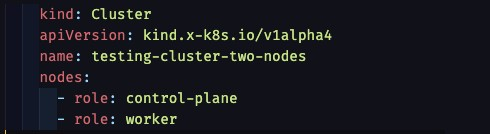
\includegraphics[width=1\textwidth]{resources/chapter-4/pengujian/kubernetes-lokal-config.jpg}
  \caption{Konfigurasi Pembuatan \textit{Kubernetes Testing Cluster} Dengan Kakas \textit{Kind}}
  \label{fig:kubernetes-lokal-config-testing}
\end{figure}

Setelah itu jalankan perintah "kind create cluster --config testing-cluster.yaml" untuk membuat \textit{cluster} pada \textit{docker}. Hasil dari perintahh ini yaitu tercipta dua buah \textit{container} pada \textit{docker} yang memiliki peran \textit{master} dan \textit{slave} seperti pada gambar \ref{fig:kubernetes-lokal-config-testing-result}.

\begin{figure}[ht]
  \centering
  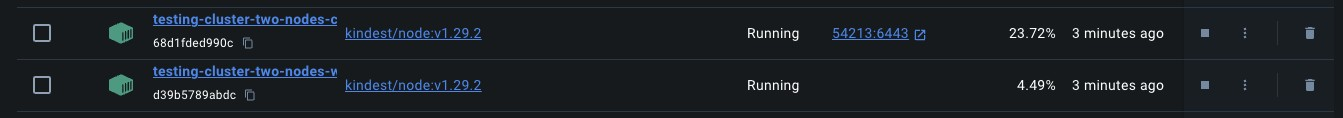
\includegraphics[width=1\textwidth]{resources/chapter-4/pengujian/kubernetes-lokal-config-result.jpg}
  \caption{Hasil \textit{Kubernetes Testing Cluster} pada \textit{Docker}}
  \label{fig:kubernetes-lokal-config-testing-result}
\end{figure}

\subsubsection{Kubernetes GCP}
\label{subsubsec:kubernetes-gcp}
Pada lingkungan ini dibuat dua buah \textit{compute engine (virtual machine)} pada \textit{GCP}. Masing masing dari \textit{virtual machine} berperan sebagai kubernetes \textit{cluster} yang bernama \textit{prod-cluster-example}.

\begin{enumerate}
  \item Buat dua \textit{virtual machine} pada \textit{compute engine GCP} dengan spesifikasi berikut. Hasil pembuatan \textit{virtual machine} dapat dilihat pada lampiran \ref{fig:hasil-pembuatan-virtual-machine-gcp}
        \begin{enumerate}
          \item Ubuntu 24.04
          \item 2GB Memory
          \item 10GB Storage Persistent Disk
          \item 0.5 - 2Vcpu (1 shared core)
          \item Region Asia southeast2-c
        \end{enumerate}
  \item Membuat \textit{Firewall Rule} Untuk membuka port yang digunakan oleh Kubernetes. Untuk daftar opsi setiap port yang dibuka dapat dilihat pada lampiran \ref{fig:daftar-kegunaan-port}. Untuk hasil pembuatan firewall dapat dilihat pada lampiran \ref{fig:hasil-firewall-rule-pada-gcp}
  \item Konfigurasi \textit{gare-test-kubernetes-server} sebagai master nodes. Konfigurasi dilakukan dengan cara mengunduh instalasi dari k3s dengan perintah seperti pada lampiran \ref{fig:instalasi-master-node-gcp}.
  \item Konfigurasi virutal machine lainnya yaitu \textit{gare-test-kubernetes-server-node} sebagai \textit{worker node}. Untuk meregistrasi \textit{node} ke dalam \textit{cluster} perlu adanya autentikasi untuk memasitikan hanya \textit{node} yang benar yang boleh masuk ke dalam \textit{cluster}. K3s memiliki token generator yang dapat digunakan untuk mencegah akses yang tidak diinginkan, registrasi token dapat dilihat pada lampiran \ref{fig:pengambilan-token-registrasi-cluster}. Token tersebut digunakan untuk meregistrasi \textit{node} ini ke \textit{master} dengan \textit{public ip} node tersebut. Ilustrasi dapat dilihat pada lampiran \ref{fig:instalasi-worker-node-gcp}.
  \item Ambil konfigurasi \textit{cluster} di \textit{master node} dan pindahkan ke lokasi \textit{server berjalan} untuk meregistrasi \textit{cluster} ke dalam sistem. Setelah melakukan kelima langkah ini \textit{cluster} sudah terintegrasi dengan sistem. Ilustrasi pemindahan konfigurasi dapat dilihat pada lampiran \ref{fig:konfigurasi-cluster-master-node-gcp} dan \ref{fig:proses-pemindahan-konfigurasi-master-gcp}.
\end{enumerate}

\subsubsection{Kubernetes RaspberryPi}
Pada lingkungan ini dibuat cluster dengan dua nodes pada RaspberryPi. Cluster yang dibuat bernama cluster-raspi yang memiliki spesifikasi hardware RaspberryPi berikut.

\begin{enumerate}
  \item Master node menggunakan Raspberry Pi 3 Model B Rev 1.2 dengan 1GB RAM dan 4 CPU @ 1.2GHz dengan hostname masterpi. Informasi lebih lengkap dapat dilihat pada lampiran \ref{fig:hostname-raspi-master-nodes} dan \ref{fig:spesifikasi-raspi-master-nodes}
  \item Worker node menggunakan Raspberry Pi 2 Model B Rev 1.1 dengan 1GB RAM dan 4 CPU @ 900MHz dengan hostname raspberrypi. Informasi lebih lengkap dapat dilihat pada lampiran \ref{fig:hostname-raspi-worker-nodes} dan \ref{fig:spesifikasi-raspi-worker-nodes}
\end{enumerate}

Berikut merupakan tata cara pembuatan cluster kubernetes pada \textit{RaspberryPi}. Diasumsikan \textit{device} \textit{RaspberryPi} sudah terhubung ke dalam jaringan yang sama sehingga tidak perlu \textit{port forwarding} / \textit{public ip}.

\begin{enumerate}
  \item Konfigurasi \textit{hostname masterpi} sebagai master nodes. Perlu dilakukan konfigurasi tambahan untuk menambahkan cgroups pada raspberrypi karena secara default opsi ini \textit{disabled}. cgroups merupakan kepanjangan dari \textit{Control Groups} yang berfungsi sebagai \textit{resource management} pada linux dan digunakan dalam proses kontainerisasi. Selanjutnya mirip serperti konfigurasi pada bagian \ref{subsubsec:kubernetes-gcp}, perlu mengunduh instalasi dari k3s dengan perintah seperti pada lampiran \ref{fig:instalasi-master-raspi-nodes}.
  \item Konfigurasi \textit{node} lainnya yaitu \textit{hostname raspberrypi} sebagai \textit{worker node}. Untuk meregistrasi \textit{node} ke dalam \textit{cluster} perlu adanya autentikasi untuk memasitikan hanya \textit{node} yang benar yang boleh masuk ke dalam \textit{cluster}. K3s memiliki token generator yang dapat digunakan untuk mencegah akses yang tidak diinginkan, registrasi token dapat dilihat pada lampiran \ref{fig:raspi-master-gen-token}. Token tersebut digunakan untuk meregistrasi \textit{node} ini ke \textit{master} dengan \textit{ip local} node master. Ilustrasi dapat dilihat pada lampiran \ref{fig:instalasi-worker-raspi-node}.
  \item Ambil konfigurasi \textit{cluster} di \textit{master node} dan pindahkan ke lokasi \textit{server berjalan} untuk meregistrasi \textit{cluster} ke dalam sistem. Setelah melakukan langkah ini \textit{cluster} sudah terintegrasi dengan sistem. Ilustrasi pemindahan konfigurasi dapat dilihat pada lampiran \ref{fig:raspi-kube-config} dan \ref{fig:raspi-add-kubeconfig}.
\end{enumerate}

\subsection{Pengujian Komponen}
Pengujian di level komponen memastikan bahwa seluruh fungsionalitas yang tidak melibatkan servis eksternal di dalam komponen bekerja dengan baik. Pengujian ini dibagi menjadi beberapa bagian sesuai dengan domain yang telah dijelaskan pada bagian \ref{subsec:implementasi-service}. Pada masing masing domain terdapat tabel yang memetakan hubungan antara kebutuhan fungsional serta pengujian yang bersesuaian. Pengujian dilakukan menggunakan lingkungan lokal dengan nama cluster "kind-testing-cluster-two-nodes"

\subsubsection{Fungsionalitas pada Domain Company}

Pengujian dengan ID P01 dilakukan dengan skenario yaitu admin berhasil membuat \textit{company} baru dengan nama \textit{cluster} yang tersedia pada sistem. Tersedia artinya konfigurasi kubernetes \textit{cluster} terdapat pada kubernetes \textit{config server}. Daftar \textit{cluster name} yang tersedia dapat dilihat pada lampiran \ref{fig:list-cluster-tersedia}. Admin membuat request dengan Postman kepada \textit{server} dengan request seperti berikut.

\begin{enumerate}
  \item Mengisi \textit{field name} dengan nilai "new company"
  \item Mengisi \textit{field cluster\textunderscore name} dengan nilai "kind-testing-cluster-two-nodes"
\end{enumerate}

\textit{Request} dibuat dengan membuat request menggunakan Postman pada url /admin-api/v1/companies dengan metode POST. \textit{Request dan Response} dapat dilihat pada lampiran \ref{fig:pengujian-p01}

Pengujian dengan ID P02 dilakukan dengan skenario yaitu admin tidak berhasil membuat \textit{company} karena nama cluster yang tidak tersedia pada server. Tersedia berarti, konfigurasi kubernetes cluster terdapat pada kubernetes \textit{config server} Admin membuat request dengan Postman kepada server dengan request seperti berikut.

\begin{enumerate}
  \item Mengisi \textit{field name} dengan nilai "new company"
  \item Mengisi \textit{field cluster\textunderscore name} dengan nilai "kind-testing-cluster-two-node"
\end{enumerate}

\textit{Request} dibuat dengan membuat request menggunakan Postman pada url /admin-api/v1/companies dengan metode POST. \textit{request dan response} dapat dilihat pada lampiran \ref{fig:pengujian-p02}


Pengujian dengan ID P03 dilakukan dengan skenario yaitu admin ingin mendapatkan seluruh \textit{company} yang terdaftar pada sistem. Admin membuat GET request dengan Postman ke url /admin-api/v1/companies. \textit{Response} balikan dari \textit{request} dapat dilihat pada lampiran \ref{fig:pengujian-p03}

Pengujian dengan ID P04 dilakukan dengan skenario yaitu admin ingin menghapus \textit{company} dengan id tertentu dari daftar \textit{company} pada sistem. Admin membuat DELETE request dengan Postman ke url /admin-api/v1/companies/:id. Untuk itu dibuat sebuah \textit{company} baru dengan spesifikasi sebagai berikut.

\begin{enumerate}
  \item Mengisi \textit{field name} dengan nilai "new company"
  \item Mengisi \textit{field cluster\textunderscore name} dengan nilai "kind-psa-with-cluster-pss"
\end{enumerate}

Hasil pembuatan \textit{company} dapat dilihat pada lampiran \ref{fig:pengujian-p04-1}. Admin menggunakan id company yang berhasil dibuat sesuai dengan lampiran \ref{fig:pengujian-p04-1} sebagai parameter untuk \textit{company} yang dihapus. \textit{Request dan Response} dapat dilihat pada lampiran \ref{fig:pengujian-p04}.

Seluruh rekap pengujian pada domain \textit{company} dapat dilihat pada lampiran \ref{tab:pengujian-domain-company}. Berdasarkan hasil yang diperoleh, terbukti bahwa kebutuhan fungsional dengan ID F01, F02, dan F03 telah terimplementasi dengan baik.

\subsubsection{Fungsionalitas pada Domain User}

Pengujian dengan ID P05 dilakukan dengan skenario yaitu admin berhasil membuat \textit{user} baru dengan nama, email, password, serta companyId yang valid. Admin membuat request dengan Postman kepada \textit{server} dengan request seperti berikut.

\begin{enumerate}
  \item Mengisi \textit{field name} dengan nilai "new user"
  \item Mengisi \textit{field email} dengan nilai "newuser@gmail.com"
  \item Mengisi \textit{field password} dengan nilai "inicontohpasswordges"
  \item Mengisi \textit{field company\textunderscore id} dengan nilai yang telah didapat sebelumnya yaitu "d6c03902-3758-47bd-994d-616e1917cc61"
\end{enumerate}

\textit{Request} dibuat dengan membuat request menggunakan Postman pada url /admin-api/v1/users dengan metode POST. \textit{Request dan response} dapat dilihat pada lampiran \ref{fig:pengujian-p05}

Pengujian dengan ID P06 dilakukan dengan skenario yaitu admin ingin menghapus \textit{user} dengan id tertentu dari daftar \textit{user} pada sistem. Admin membuat DELETE request dengan Postman ke url /admin-api/v1/users/:id. Admin menggunakan id user yang berhasil dibuat sesuai dengan lampiran \ref{fig:pengujian-p05} sebagai parameter untuk \textit{user} yang dihapus. \textit{Request dan Response} dapat dilihat pada lampiran \ref{fig:pengujian-p06}.

Pengujian dengan ID P07 dilakukan dengan skenario yaitu user ingin login ke dalam sistem. Langkah langkah yang dilakukan:

\begin{enumerate}
  \item Mengunjungi halaman /login
  \item Memasukan \textit{field email} dengan "raspi@gmail.com"
  \item Memasukan \textit{field password} dengan "inicontohpasswordges"
  \item Kilk tombol "login"
\end{enumerate}

Setelah seluruh langkah dilakukan, muncul sebuah modal pada kanan bawah dengan pesan "sucess login, redirecting" serta redirect ke halaman / yang menunjukan bahwa proses login telah berhasil. Hasil dapat dilihat pada lampiran \ref{fig:pengujian-p07}

Pengujian dengan ID P08 dilakukan dengan skenario yaitu user ingin login ke dalam sistem dengan kredensial yang tidak valid. Langkah langkah yang dilakukan:

\begin{enumerate}
  \item Mengunjungi halaman /login
  \item Memasukan \textit{field email} dengan "raspi@gmail.co"
  \item Memasukan \textit{field password} dengan "inicontohpasswordge"
  \item Kilk tombol "login"
\end{enumerate}

Setelah seluruh langkah dilakukan, muncul sebuah modal pada kanan bawah dengan pesan "invalid combination email or password". Dengan adanya modal ini \textit{user} menjadi \textit{aware} bahwa proses login yang dilakukan gagal dan perlu melakukan pengecekan kembali input yang dimasukkan. Hasil dapat dilihat pada lampiran \ref{fig:pengujian-p08}

Pengujian dengan ID P09 dilakukan dengan skenario yaitu user ingin logout dari sistem. Pengujian dilakukan dengan cara menekan tombol logout pada bagian kiri bawah \textit{sidebar}. Setelah itu cookie dihapus dan dilakukan \textit{redirect} ke /login page.

Pengujian dengan ID P10, P11 dilakukan dengan skenario yaitu setelah \textit{user} berhasil login, \textit{user} ingin mendapatkan informasi detail \textit{company} serta seluruh \textit{user} pada \textit{company} tersebut dengan mengunjungi halaman /account. Halaman ini dapat dikunjungi dengan cara menekan tombol "account" pada sidebar. Hasil dapat dilihat pada lampiran \ref{fig:pengujian-p08-09}.

Seluruh rekap pengujian pada domain \textit{user} dapat dilihat pada lampiran \ref{tab:pengujian-domain-user}. Berdasarkan hasil yang diperoleh, terbukti bahwa kebutuhan fungsional dengan ID F04 hingga F09 telah terimplementasi dengan baik.
\subsubsection{Fungsionalitas pada Domain \textit{Device}}

Pengujian dengan ID P12 dilakukan dengan skenario \textit{user} yang telah terautentikasi ingin menambahkan \textit{device} yang dia miliki ke dalam sistem dengan \textit{node name} yang valid. Langkah langkah yang dilakukan:
\begin{enumerate}
  \item Mengunjungi halaman /devices
  \item Menekan tombol "Add Device"
  \item Mengisi \textit{field name} dengan "raspi-device-1"
  \item Mengisi \textit{field node name} dengan "testing-cluster-two-nodes-control-plane"
  \item Mengisi \textit{field type} dengan nilai "raspi"
  \item Mengisi label dengan "testing=true"
\end{enumerate}

Setelah pengujian dilakukan, muncul deskripsi \textit{device} yang telah dibuat pada tabel yang sebelumnya kosong. Pada bagian kanan bawah juga terdapat modal yang menunjukan bahwa pembuatan \textit{device} berhasil. Hasil dapat dilihat pada lampiran \ref{fig:pengujian-p12-success}.

Pengujian dengan ID P13 dilakukan skenario \textit{user} yang telah terautentikasi ingin menambahkan \textit{device} yang dia miliki ke dalam sistem dengan \textit{node name} yang tidak terdapat pada \textit{cluster}. Langkah langkah yang dilakukan:
\begin{enumerate}
  \item Mengunjungi halaman /devices
  \item Menekan tombol "Add Device"
  \item Mengisi \textit{field name} dengan "raspi-device-1"
  \item Mengisi \textit{field node name} dengan "testing-cluster-two-nodes-control-plan"
  \item Mengisi \textit{field type} dengan nilai "raspi"
  \item Mengisi label dengan "testing=true"
\end{enumerate}

Setelah pengujian dilakukan, muncul sebuah modal pada bagian kanan bawah juga terdapat modal yang menunjukan bahwa pembuatan \textit{device} gagal dengan pesan "node not found". Hasil dapat dilihat pada lampiran \ref{fig:pengujian-p12-failed}.

Pengujian dengan ID P14 dilakukan dengan skenario \textit{user} ingin melihat seluruh \textit{device} yang \textit{company} miliki. Pengujian ini dilakukan dengan cara mengunjungi halaman /devices dan melihat isi dari tabel yang tersedia. Berdasarkan pengujian P11 dapat dilihat bahwa tabel terisi dengan nilai \textit{device} yang telah dibuat, hal ini menunjukan bahwa \textit{user} dapat melihat perangkat yang \textit{company} miliki.

Pengujian dengan ID P15 dilakukan dengan skenario \textit{user} ingin menghapus salah satu \textit{device} yang ia miliki. Langkah langkah yang dilakukan:
\begin{enumerate}
  \item Mengunjungi halaman /devices
  \item Menekan tombol "titik tiga (\textit{elipsis horizontal})" yang berada pada ujung tabel
  \item Menekan tombol "delete" dari popup modal
\end{enumerate}

Setelah melakukan langkah langkah tersebut dapat dilhat bahwa tidak ada data pada tabel. Hal ini menunjukan bahwa \textit{device} berhasil dihapus dari sistem. Hasil pengujian dapat dilihat pada lampiran \ref{fig:pengujian-p15}.

Seluruh rekap pengujian pada domain \textit{devices} dapat dilihat pada lampiran \ref{tab:pengujian-domain-device}. Berdasarkan hasil yang diperoleh, terbukti bahwa kebutuhan fungsional dengan ID F10 hingga F15 telah terimplementasi dengan baik.

\subsubsection{Fungsionalitas pada Domain \textit{Groups}}

Pengujian dengan ID P16 dilakukan dengan skenario \textit{user} ingin membuat \textit{group} baru dengan nama "group-baru" pada sistem. Langkah langkah yang dilakukan:
\begin{enumerate}
  \item Mengunjungi halaman /groups
  \item Menekan tombol "Add Group" pada bagian kanan bawah
  \item Mengisi \textit{field name} dengan nilai "group-baru"
  \item Menekan tombol "submit"
\end{enumerate}

Setelah pengujian dilakukan, tabel yang awalnya kosong terisi dengan deskripsi \textit{group} yang telah dibuat. Selain itu, terdapat modal pada bagian bawah kanan yang menunjukan bahwa pembuatan \textit{group} telah berhasil. Hasil dari pengujian dapat dilihat pada lampiran \ref{fig:pengujian-p16}

Pengujian dengan ID P17 dilakukan dengan skenario \textit{user} ingin membuat \textit{group} baru dengan nama yang duplikat pada sistem. Langkah langkah yang dilakukan:
\begin{enumerate}
  \item Mengunjungi halaman /groups
  \item Menekan tombol "Add Group" pada bagian kanan bawah
  \item Mengisi \textit{field name} dengan nilai "group-baru"
  \item Menekan tombol "submit"
\end{enumerate}

Setelah pengujian dilakukan, muncul modal pada bagian bawah kanan yang menunjukan bahwa pembuatan \textit{group} gagal. Pesan yang tidunjukan yaitu "group-baru is exists please another name". Hasil dari pengujian dapat dilihat pada lampiran \ref{fig:pengujian-p17}

Pengujian dengan ID P18 dilakukan dengan skenario \textit{user} ingin melihat daftar \textit{group} yang tersedia pada sistem. Pengujian ini dilakukan dengan cara mengunjungi halaman /groups. Dapat dilihat dari pengujian P17 bahwa tabel \textit{groups} terisi dengan nilai yang sudah dibuat sebelumnya. Hal ini menunjukan bawha \textit{user} dapat melihat daftar \textit{groups} pada sistem.

Pengujian dengan ID P19 dilakukan dengan skenario \textit{user} ingin menghapus salah satu \textit{group} yang dimiliki. Langkah langkah yang dilakukan:
\begin{enumerate}
  \item Mengunjungi halaman /groups
  \item Menekan tombol "titik tiga (\textit{elipsis horizontal})" yang berada pada ujung tabel
  \item Menekan tombol "delete" dari popup modal
\end{enumerate}

Setelah melakukan langkah langkah tersebut dapat dilhat bahwa tidak ada data pada tabel. Hal ini menunjukan bahwa \textit{device} berhasil dihapus dari sistem. Hasil pengujian dapat dilihat pada lampiran \ref{fig:pengujian-p19}.

\subsection{Pengujian Sistem}
Pengujian sistem memiliki kaitan dengan satu atau lebih domain dan fungsionalitas. Pengujian ini dibagi menjadi dua bagian yaitu pengujian pada \textit{cluster GCP} serta pengujian pada \textit{cluster RaspberryPi} yang dibagi berdasarkan abstrasksi kebutuhan utama yaitu melakukan \textit{remote deployment}.


\subsubsection{Pengujian LED Blink pada RaspberryPi}

Pengujian sistem ini mencakup pengujian dengan ID P20, P21, P22, P23, P24, P25, P26, P27, P28, P29, P30 dan P31. Pada pengujian sistem ini, dilakukan proses \textit{remote deployment} untuk menyalakan lampu blink pada RaspberryPi dengan cluster "cluster-raspi". Dibuat sebuah script python yang berinteraksi dengan GPIO pada pin 2 untuk menyalakan lampu LED. Script dapat dilihat pada lampiran \ref{fig:raspi-python-led-script}

\begin{figure}[ht]
  \centering
  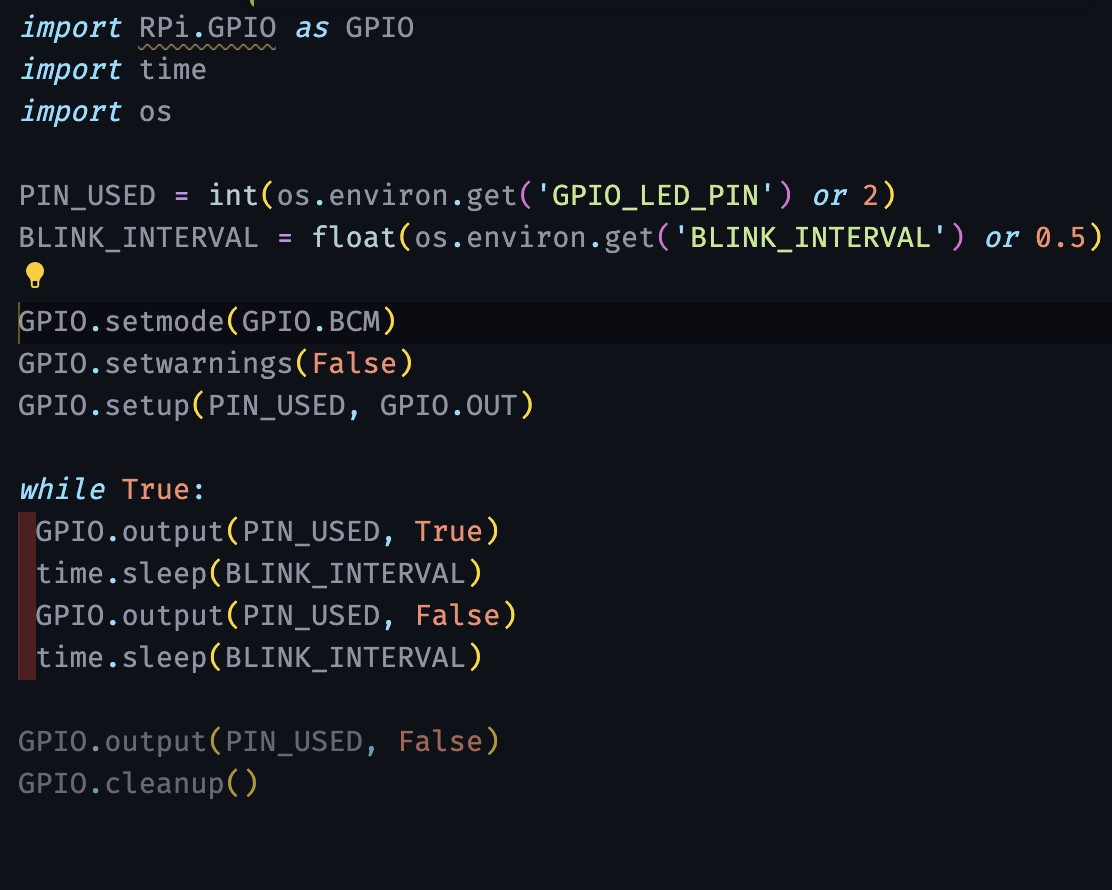
\includegraphics[width=0.8\textwidth]{resources/chapter-4/pengujian/pengujian-sistem-raspi-09-led.jpg}
  \caption{Python Raspi LED Script}
  \label{fig:raspi-python-led-script}
\end{figure}

Dari script tersebut, dibuat docker image dengan base image armv7 yang membungkus python tersebut agar dapat berjalan di sistem IoT. Docker image yang telah dibuat diunggah ke dockerhub dengan nama {gawrgare/led\textunderscore blink}. Isi dari dockerfile dapat dilihat pada lampiran \ref{fig:raspi-docker-led-script}. Setelah docker image tersedia, selanjutnya terdapat beberapa langkah yang harus disiapkan sebelum melakukan \textit{deployment} pada lingkungan raspberrypi.

\begin{enumerate}
  \item Membuat \textit{company} dengan nama "raspi-company" dan \textit{cluster\textunderscore name} "cluster-raspi". Hasil dapat dilihat pada lampiran \ref{fig:pengujian-sistem-raspi-01}
  \item Membuat user pada \textit{company} tersebut dengan email \textit{raspi@gmail.com}. Hasil dapat dilihat pada lampiran \ref{fig:pengujian-sistem-raspi-02}
  \item Login dengan kredensial yang telah dibuat
  \item Mengunjungi halaman /devices dan melakukan registrasi \textit{devices} untuk kedua RaspberryPi dengan daftar nama nodes yang dapat dilihat pada lampiran \ref{fig:pengujian-sistem-raspi-04}
        \begin{enumerate}
          \item \textit{Device} "raspi-master" untuk \textit{hostname masterpi} dengan nama \textit{cluster} yaitu "master-node-raspi"
          \item  \textit{Device} "raspi-worker" untuk \textit{hostname raspberrypi} dengan nama \textit{cluster} yaitu "worker-node-raspi"
        \end{enumerate}
  \item Mengunjungi halaman /groups dan membuat \textit{group} "raspi-group-blink". Hasil dapat dilihat pada lampiran \ref{fig:pengujian-sistem-raspi-05}
  \item Mengunjungi halaman group detail "raspi-group-blink" lalu menambahkan kedua device ke dalam group.
  \item Mengunjungi halaman \textit{deployment} lalu membuat repository dengan nama "raspi-image-blink" dan image\textit{ gawrgare/led\textunderscore blink}.
  \item Membuat deployment dengan nama "raspi-deployment-blink" dan mengisi target dengan "node=master" pada halaman \textit{deployment}.
\end{enumerate}

Layout dari RaspberryPi serta letak kabel dan LED dapat dilihat pada lampiran \ref{fig:pengujian-sistem-raspi-layout}. Setelah semua persiapan dilakukan, dilakukan pengujian dengan dua jenis \textit{deployment} yaitu \textit{target} dan \textit{custom} dengan versi \textit{group}.
\begin{enumerate}
  \item Target deployment merupakan deployment yang dilakukan sesuai dengan nilai target pada deployment object, dalam kasus ini target nya ialah node dengan attribut "node=master". Pengujian tipe ini hanya melakukan deployment dengan \textit{hostname masterpi} yang memiliki nama node "master-node-raspi". Setelah deployment dilakukan, LED yang terhubung dengan pin pada "master-node-raspi" berkedip, hal ini menunjukan bahwa proses deployment telah berhasil dilakukan. Hasil dapat dilihat pada lampiran \ref{fig:hasil-pengujian-sistem-raspi-target}.
  \item Custom deployment mengabaikan nilai target yang terdapat pada objek deployment dan melakukan deployment sesuai jenis serta id yang diinginkan. Terdapat dua jenis yaitu \textit{group} dan \textit{device}. Dalam kasus groups, Deployment dilakukan ke dua \textit{device} yang terhubung ke \textit{group} "raspi-group-blink". Setelah deployment dilakukan, kedua LED berkedip menunjukan bahwa script berhasil dijalankan untuk setiap \textit{device} yang terhubung pada group. Hasil dapat dilihat pada lampiran \ref{fig:hasil-pengujian-sistem-raspi-custom}.
\end{enumerate}

Setelah deployment berhasil dilakukan, pengujian dilanjutkan dengan mengunjungi halaman detail dari "raspi-deployment-blink" untuk melihat riwayat deployment. Hasil dapat dilhat pada lampiran \ref{fig:pengujian-sistem-raspi-10}. Dapat dilihat bahwa pengujian dengan ID P20 hingga P31 menunjukan hasil yang sesuai dengan kebutuhan fungsional yang telah didefinisikan. Seluruh rekap pengujian sistem ini dapat dilihat pada lampiran \ref{tab:pengujian-sistem-raspi}.
\subsubsection{Penguijan Deployment MQTT Client untuk Mengirim data Temperatur pada \textit{Clutser GCP}}

Pengujian ini mencakup pengujian dengan ID P32 hingga P39. Pada pengujian sistem ini, dilakukan proses \textit{remote deployment} MQTT pada \textit{cluster GCP} dengan cluster name "prod-cluster-example". Pengujian ini dilakukan untuk mensimulasikan node sebagai sebuah sensor temperatur yang akan mengirimkan data sensornya melalui mqtt client ke mqtt broker. Pengujian ini membuktikan  \textit{compatibility} dari sistem yang tidak terbatas pada IoT namun seluruh perangkat yang berbasis UNIX yang dapat menjalankan kubernetes. Proses \textit{remote deployment} dilakukan dengan menggunakan image gawrgare/mqtt-client yang telah dibuat dan di \textit{publish} pada \textit{dockerhub}. Script yang digunakan untuk membuat image docker dibuat dengan python serta akan mengirimkan data dalam interval 5 detik. \textit{Script} dapat dilihat pada gambar \ref{fig:pengujian-gcp-script-docker-images}

\begin{figure}[ht]
  \centering
  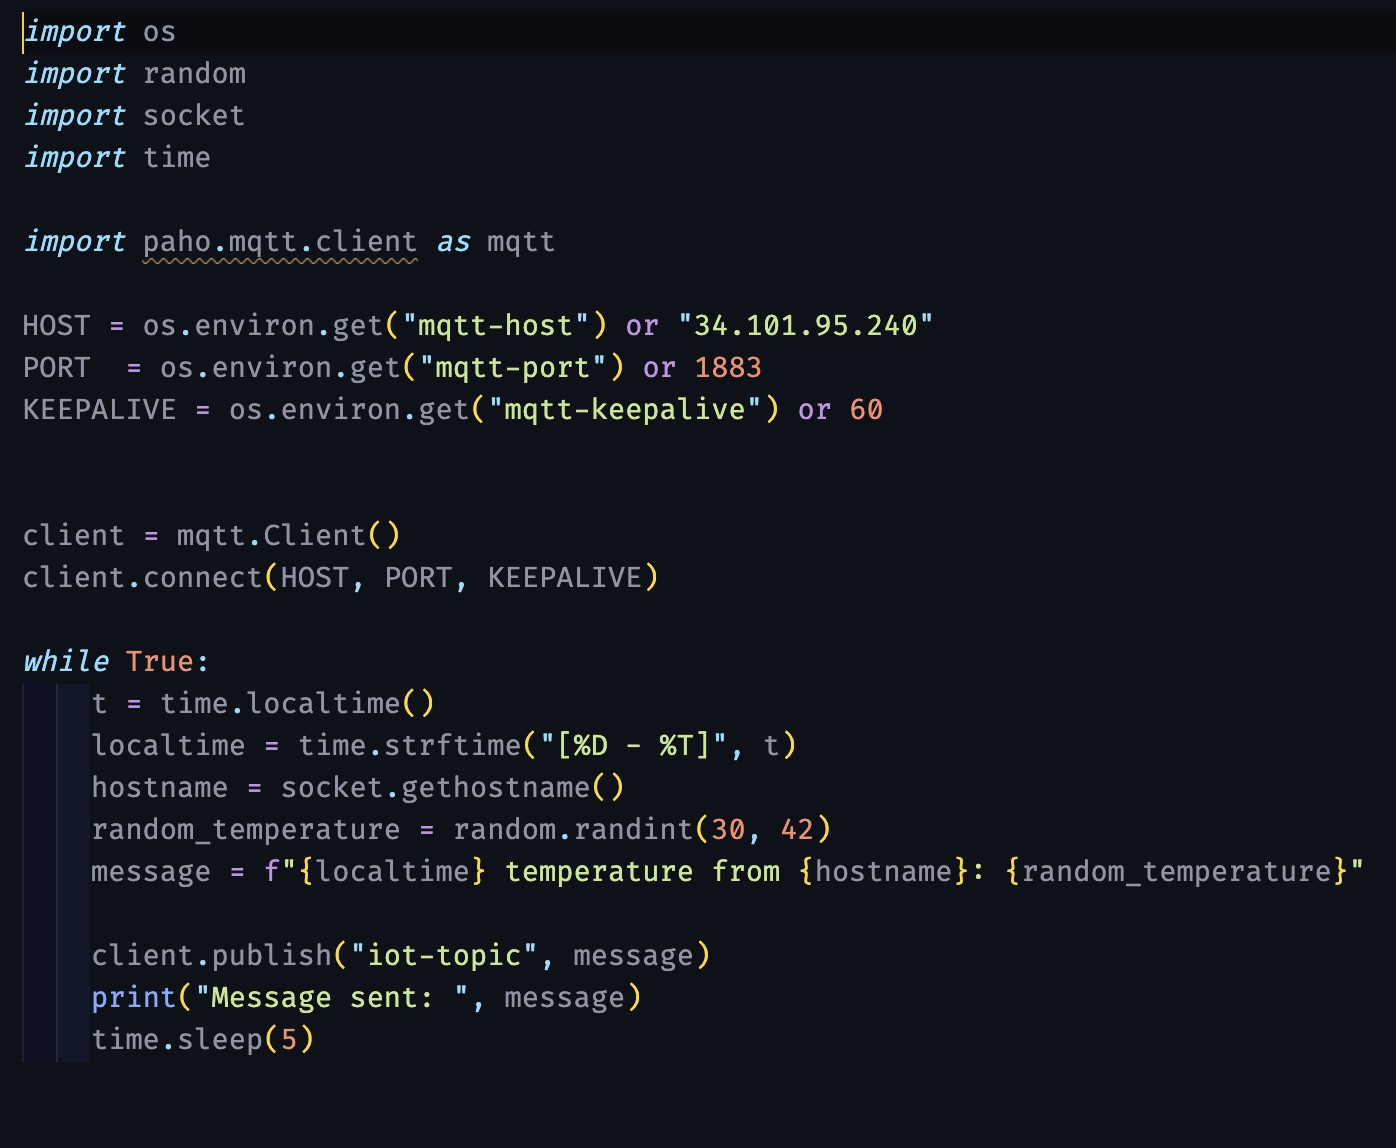
\includegraphics[width=0.8\textwidth]{resources/chapter-4/pengujian/pengujian-gcp-docker-image.jpg}
  \caption{Script MQTT Client untuk Docker Image gawrgare/mqtt-client}
  \label{fig:pengujian-gcp-script-docker-images}
\end{figure}

Pengujian dilakukan dengan mengikuti langkah langkah berikut:

\begin{enumerate}
  \item Melakukan setup mqtt-broker pada server yang memiliki IP 34.101.95.240.
  \item Membuat \textit{company} "test-semhas" dan nama cluster "prod-cluster-example". Hasil dapat dilihat pada lampiran \ref{fig:pengujian-sistem-gcp-01}
  \item Membuat \textit{user} dengan email "test@gmail.com", nama "test-user-semhas". Hasil dapat dilihat pada lampiran \ref{fig:pengujian-sistem-gcp-02}
  \item Login dengan menggunakan kredensial "test@gmail.com". Hasil dapat dilihat pada lampiran \ref{fig:pengujian-sistem-gcp-03}
  \item Mengunjungi halaman /devices lalu membuat \textit{device} "raspberrypi-pi-1" dan nama \textit{node} "master-cluster" serta memiliki label "sukses=aamiin". Hasil dapat dilihat pada lampiran \ref{fig:pengujian-sistem-gcp-04}
  \item Mengunjungi halaman /deployments lalu membuat \textit{deployment plan} untuk v1 dengan mengambil repository "gawrgare/mqtt-client" serta memiliki nama "mqtt-deployment". Hasil dapat dilihat pada lampiran \ref{fig:pengujian-sistem-gcp-05}
  \item Mengunjungi halaman /remote-deployment lalu melakukan \textit{deployment} dengan tipe "TARGET". Hasil dapat dilihat pada lampiran \ref{fig:pengujian-sistem-gcp-06}
  \item Setelah deployment berhasil dilakukan, hapus \textit{deployment} yang telah dibuat. Hasil dapat dilihat pada lampiran \ref{fig:pengujian-sistem-gcp-07}.
  \item Setelah deployment berhasil dibuat, jalankan kode untuk mengkonsumsi data dari mqtt-broker yang dikirimkan dari hasil deployment. Hasil dapat dilihat pada lampiran \ref{fig:pengujian-sistem-gcp-sukses-mqtt}
  \item Mengunjungi halaman /deployments lalu menghapus \textit{deployment plan} dengan nama "mqtt-deployment". Hasil dapat dilihat pada lampiran \ref{fig:pengujian-sistem-gcp-08}
  \item Mengunjungi halaman /deployments lalu menghapus \textit{deployment image} dengan nama "deploy-mqtt-client". Hasil dapat dilihat pada lampiran \ref{fig:pengujian-sistem-gcp-09}
\end{enumerate}

Setelah seluruh langkah dilakukan, pengujian dengan ID P32 hingga P39 berhasil diimplementasikan. Seluruh rekap pengujian dapat dilihat pada lampiran \ref{tab:pengujian-sistem-gcp}.

\subsubsection{Pengujian Gagal deployment}
Pengujian ini mencakup pengujian dengan ID40 hingga P46. Pada pengujian sistem ini, dilakukan proses \textit{Remote Deployment} yang gagal. Gagal berarti \textit{deployment} berhasil dilakukan dengan baik namun aplikasi gagal untuk dijalankan. Kegagalan dapat disebabkan oleh dua hal yaitu:
\begin{enumerate}
  \item Tidak ada \textit{device} yang memiliki label yang sesuai dengan target \textit{deployment}
  \item \textit{Image} yang tidak tersedia pada \textit{dockerhub}
\end{enumerate}
Pengujian ini akan mencakup kedua kegagalan yaitu dibuat \textit{deployment} dengan label yang tidak ada serta \textit{deployment} dengan image yang tidak ada pada \textit{dockerhub}. Ketika terjadi kegagalan proses \textit{deployment} akan secara otomatis dihapus karena terdapat sebuah \textit{asynchronus checking} setiap 10 detik dan sebuah timeout selama 200 detik yang membatasi waktu proses \textit{deployment}.

Pengujian kegagalan label dilakukan dengan mengikuti langkah langkah berikut:

\begin{enumerate}
  \item Login dengan menggunakan kredensial "test@gmail.com" dan password yaitu "inicontohpasswordges". Hasil dapat dilihat pada lampiran \ref{fig:pengujian-sistem-gagal-00}
  \item Mengunjungi halaman /deployments lalu buat \textit{deployment plan} dengan nama repository "deploy-mqtt-client" dengan v1 dan nama "deployment-plan-mqtt-client-failed" serta memiliki label "temperature=false". Hasil dapat dilihat pada lampiran \ref{fig:pengujian-sistem-gagal-01}
  \item Mengunjungi halaman /remote-deployment lalu melakukan \textit{deployment} dengan plan sebelumnya serta memiliki tipe "TARGET"
  \item \textit{Deployment} akan gagal karena tidak terdapat \textit{device} dengan label yang sesuai dengan \textit{deployment plan} Hasil dapat dilhat pada lampiran \ref{fig:pengujian-sistem-gagal-02}
  \item \textit{Program} akan melakukan \textit{polling} setiap 10 detik. Lalu setelah 200 detik \textit{deployment} akan dihapus, menandakan bahwa terdapat kegagalan pada \textit{deployment}. Hasil dapat dilhat pada lampiran \ref{fig:pengujian-sistem-gagal-03}
\end{enumerate}

Kegagalan pada kasus ini, disebabkan label pada deployment yang menargetkan "temperature=false" sedangkan kedua \textit{device} yang ada tidak memiliki label tersebut. Sehingga \textit{scheduler} pada kubernetes tidak bisa membuat \textit{deployment} dan sistem menghapus \textit{deployment} setelah melewati waktu \textit{timeout} 200 detik.

Selanjutnya, Pengujian kegagalan image dilakukan dengan mengikuti langkah langkah berikut:

\begin{enumerate}
  \item Login dengan menggunakan kredensial "test@gmail.com" dan password yaitu "inicontohpasswordges". Hasil dapat dilihat pada lampiran \ref{fig:pengujian-sistem-gagal-01}
  \item Mengunjungi halaman /deployments lalu membuat repository dengan image "nonexist-image". Hasil dapat dilihat pada lampiran \ref{fig:pengujian-sistem-gagal-06}
  \item Pada halaman yang sama, buat \textit{deployment plan} dengan repository yang telah dibuat dengan v1 dan nama "deployment-image" serta memiliki label "sukses=aamiin". Hasil dapat dilihat pada lampiran \ref{fig:pengujian-sistem-gagal-07}
  \item Mengunjungi halaman /remote-deployment lalu melakukan \textit{deployment} dengan plan sebelumnya serta memiliki tipe "TARGET"
  \item \textit{Deployment} akan gagal karena tidak menemukan image "nonexist-image" pada \textit{dockerhub}. Hasil dapat dilhat pada lampiran \ref{fig:pengujian-sistem-gagal-08}
  \item \textit{Program} akan melakukan \textit{polling} setiap 10s. Lalu setelah 200 detik \textit{deployment} akan dihapus, menandakan bahwa terdapat kegagalan pada \textit{deployment}. Hasil dapat dilhat pada lampiran \ref{fig:pengujian-sistem-gagal-09}
\end{enumerate}

Kegagalan pada pengujian ini disebabkan oleh tidak tersedianya image "nonexist-image" pada \textit{dockerhub}. Hal ini menyebabkan terjadi error ketika proses \textit{deployment} yaitu ErrImagePull, yang diakibatkan error ketika mengambil image dari \textit{dockerhub} seperti pada lampiran \ref{fig:pengujian-sistem-gagal-08}. Setelah seluruh rangkaian pengujian dilakukan, pengujian dengan ID P40 hingga P46 berjalan sesuai ekspektasi. Seluruh rekap pengujian ini dapat dilihat pada lampiran \ref{tab:pengujian-sistem-gagal}

\subsection{Pengujian Non Fungsional}
Pada bagian ini, dilakukan pengujian terhadap kebutuhan non-fungsional sistem. Terdapat dua kebutuhan non-fungsional yang akan diuji yaitu \textit{Security dan Portability}. Pengujian akan menggunakan \textit{security testing} dan \textit{compatibility testing} untuk masing masing kebutuhan non-fungsional.

\subsubsection{\textit{Security Testing}}
\textit{Security Testing} bertujuan untuk menguji kebutuhan non-fungsional yaitu \textit{security}. Pengujian ini hanya terbatas pada masalah autentikasi dan authorisasi. Pengujian kebutuhan non-fungsional ini dilakukan dengan cara mencoba mengakses \textit{dashboard} dan \textit{service} tanpa meletakan token yang valid. Pengujian ini mencakup ID pengujian P47 hingga P50

\begin{enumerate}
  \item Mengakses \textit{dashboard} tanpa kredensial

        Ketika mengakses \textit{dashboard} tanpa memiliki kredensial, \textit{dashboard} memiliki \textit{middleware} yang akan mengecek token yang disimpan pada \textit{client}. Jika token tidak valid maka sistem akan langsung melakukan \textit{redirect} ke halaman login.

  \item Mengakses user \textit{service} tanpa kredensial

        Ketika mencoba untuk mengakses \textit{service} pada endpoint apapun, \textit{service} memiliki \textit{middleware}
        yang akan mengecek header authentikasi yang dikirimkan oleh client. Jika kredensial pada header tidak dicantumkan maka akan mengembalikan \textit{401 Unauthorized} seperti pada lampiran \ref{fig:akses-service-user}.

  \item Mengakses admin \textit{service} tanpa kredensial

        Admin endpoint memiliki \textit{middleware} validateAdminJWTKey. Ketika mencoba untuk mengakses \textit{endpoint} admin tanpa memberikan header X-Admin-Api-Key yang sesuai maka \textit{service} akan mengembalikan \textit{401 Unauthorized} seperti pada lampiran \ref{fig:akses-service-admin}.

  \item Mengakses \textit{url kubernetes} tanpa kredensial

        Seluruh cluster kubernetes akan mengexpose endpoint pada port 6443. Pengujian ini akan mengakses url kubernetes yaitu https://34.101.95.240:6443/. Ketika diakses, hasilnya akan menunjukan status \textit{401 Unauthorized} seperti pada lampiran \ref{fig:akses-service-kubernetes}.

\end{enumerate}

Setelah melakukan pengujian, pengujian dengan ID P47 hingga P50 berjalan sesuai dengan ekspektasi yaitu menunjukan kegagalan saat mengakses \textit{resource} yang diminta. Seluruh rekap pengujian dapat dilihat pada tabel \ref{tab:pengujian-nonfungsional-security}.

\subsubsection{Compatibility Testing}
\textit{Compatibility testing} dilakukan untuk menguji kebutuhan non-fungsional yaitu \textit{portability}. Pengujian kebutuhan non-fungsional ini dialkukan dengan tiga skenario yaitu mengakses \textit{dashboard} dari mobile serta mengakses dari berbagai \textit{browser}. Tujuan dari pengujian ini adalah memastikan bahwa \textit{dashboard} dapat dijalankan pada berbagai \textit{platform}. Pengujian ini mencakup pengujian dengan ID P52 hingga P54.

\begin{enumerate}
  \item Mengakses \textit{dashboard} dari perangkat mobile

        \textit{Dashboard} berhasil diakses melalui perangkat mobile dan dapat dilihat hasil dapat dilihat pada lampiran \ref{fig:akses-dashboard-mobile}.

  \item Mengakses \textit{dashboard} dari Chromium based browser

        \textit{Dashboard} berhasil diakses melalui browser \textit{chromium based} yaitu "Arc" dan "Google Chrome" yang dapat dilhat pada lampiran \ref{fig:akses-dashboard-chromium}.

  \item Mengakses \textit{dashboard} dari browser safari

        \textit{Dashboard} berhasil diakses melalui browser safari yang dapat dilhat pada lampiran \ref{fig:akses-dashboard-safari}.

\end{enumerate}

Setelah melakukan pengujian, pengujian dengan ID P51 hingga P53 berjalan sesuai dengan ekspektasi yaitu menunjukan kegagalan saat mengakses \textit{resource} yang diminta. Seluruh rekap pengujian dapat dilihat pada tabel \ref{tab:pengujian-nonfungsional-compatibility}.
Berdasarkan \textit{security testing} dan \textit{compatibility testing}, sistem \textit{remote deployment} yang dibuat telah memenuhi kebutuhan non-fungsional yang telah di definisikan pada tabel kebutuhan yang dapat dilihat pada lampiran \ref{tab:kebutuhan-non-fungsional}


